\documentclass[11pt,a4paper]{article}

\usepackage[utf8]{inputenc}
\usepackage{lmodern}
\usepackage[T1]{fontenc}
\usepackage{amsmath,amssymb,amsfonts}
\usepackage{booktabs}
\usepackage{array}
\usepackage{xcolor}
\usepackage{graphicx}
\usepackage{geometry}
\geometry{margin=2.5cm}
\usepackage{float}
\usepackage{enumitem}
\usepackage[hidelinks,pdfencoding=auto]{hyperref}
\usepackage{caption}
\usepackage{subcaption}
\usepackage{multirow}
\usepackage{setspace}
\setstretch{1.08}
\usepackage{authblk}

\newcommand{\btheta}{\boldsymbol{\theta}}
\newcommand{\bphi}{\boldsymbol{\phi}}
\newcommand{\bvarphi}{\boldsymbol{\varphi}}
\newcommand{\bpsi}{\boldsymbol{\psi}}
\newcommand{\bA}{\mathbf{A}}
\newcommand{\bb}{\mathbf{b}}
\newcommand{\Real}{\mathbb{R}}

\title{Bayesian inference of shared interaction structure\\
and patient-specific growth rates in peri-implant biofilms:\\
a 10-patient in-vivo longitudinal study}

\author[1]{Keisuke Nishioka}
\author[1]{Felix Klempt}
\author[1]{Hendrik Geisler}
\author[1]{Meisam Soleimani}
\author[2,3]{Rumjhum Mukherjee}
\author[2,3]{Szymon P. Szafra\'{n}ski}
\author[1]{Philipp Junker}
\author[2,3]{Meike Stiesch}

\affil[1]{Institute of Continuum Mechanics, Leibniz Universit\"at Hannover, Hannover, Germany}
\affil[2]{Department of Prosthetic Dentistry and Biomedical Materials Science, Hannover Medical School, Hannover, Germany}
\affil[3]{Lower Saxony Centre for Biomedical Engineering, Implant Research and Development (NIFE), Hannover, Germany}

\date{}

\begin{document}

\maketitle

\begin{abstract}
We extend the GPU-accelerated Bayesian TMCMC framework for multi-species biofilm parameter inference from controlled in-vitro conditions to a 10-patient longitudinal in-vivo dataset of peri-implant biofilm formation~\cite{Dieckow2025InVivo}.
A joint posterior over a shared $5\times5$ interaction matrix $\bA$ (15 parameters) and patient-specific intrinsic growth vectors $\bb^{(p)}$ (5 species $\times$ 10 patients\,$=\,$50 parameters; total $d\!=\!65$) is inferred by TMCMC with $N_p\!=\!1{,}000$ particles.
The MAP achieves RMSE\,$=\,$0.101 (flat prior) and 0.101 (Bergey metabolic network sign prior) on held-out week-2/3 predictions across all patients.
Cross-prediction analysis shows that the four Heine et al.\ in-vitro MAP interaction matrices~\cite{Heine2025PeriImplant} achieve RMSE\,$=\,$0.102--0.103 when combined with the Dieckow patient-specific growth rates, confirming a conserved interaction backbone between in-vitro and in-vivo settings.
Comparing sign patterns across all five conditions, three mutualistic pairs---So--An, An--Vd, and Vd--Pg---are positive in all five; the An--Vd sign reversal in the in-vivo fit is consistent with the strain substitution from \textit{V.~parvula} (in-vitro) to \textit{V.~dispar} (in-vivo).
At the community level, a 10-guild generalised Lotka-Volterra model fit to all 53 genera achieves RMSE\,$=\,$0.050 ($r=0.963$).
Integrating CLSM structural data (live-biovolume occupancy and PerLive fraction) as patient- and week-specific Hamilton ODE initial conditions reduces the guild-level Hamilton ODE RMSE by 43\,\% (0.105\,$\to$\,0.060), demonstrating that structural biofilm measurements carry independent predictive information beyond 16S composition.

\vspace{4pt}
\noindent\textbf{Keywords:}
peri-implantitis,
biofilm dynamics,
Bayesian inference,
TMCMC,
in-vivo,
multi-species interaction,
Hamilton principle,
CLSM structural data
\end{abstract}

%==============================================================================
\section{Introduction}
\label{sec:intro}
%==============================================================================

Peri-implantitis is a biofilm-driven inflammatory disease that affects 22--65\% of dental implant patients~\cite{Dieckow2025InVivo}.
The microbial communities that colonise implant surfaces are complex, patient-specific, and temporally dynamic, with recent longitudinal in-vivo characterisation~\cite{Dieckow2025InVivo} revealing that community composition evolves over the first three weeks in a highly individual manner.
Mechanistic mathematical models of biofilm dynamics provide a principled framework for quantifying these inter-species interactions from time-course data~\cite{Klempt2025ContinuumBiofilm,JunkerBalzani2021ExtendedHamilton}.

Our companion paper~\cite{NishiokaTMCMC2025} demonstrated that the extended Hamilton principle yields a 20-parameter symmetric interaction matrix~$\bA$ whose posterior can be recovered by GPU-accelerated TMCMC from in-vitro time-course data under four conditions (commensal/dysbiotic, static/HOBIC reactor).
The key biological insight was that the health-to-disease transition corresponds to a structural reorganisation of~$\bA$, not merely a parameter rescaling.

Here we address four open questions: (i) does the inferred interaction structure generalise to in-vivo conditions with patient-level heterogeneity; (ii) can a joint model that separates shared ecological interactions from patient-specific growth rates accommodate the clinical variability observed by Dieckow et al.~\cite{Dieckow2025InVivo}; (iii) can a guild-level generalised Lotka-Volterra model capture the full taxonomic diversity of the 16S data; and (iv) do CLSM structural measurements (live-biovolume occupancy, PerLive viability fraction) provide independent predictive information beyond compositional 16S data?

We answer all four questions affirmatively.
The joint model recovers a shared $\bA$ that is biologically interpretable, patient-specific $\bb^{(p)}$ that reflect individual ecological niches, and cross-prediction accuracy that rivals the Dieckow self-fit when the Heine in-vitro $\bA$ is combined with patient-specific growth rates.
A 10-guild gLV achieves $r=0.963$ covering 100\% of sequenced reads, and integrating CLSM structural data into the Hamilton ODE reduces guild-level RMSE by 43\%, a gain that is mechanistically attributable to the free-space variable $\varphi_0$ unique to the Hamilton formulation.

%==============================================================================
\section{Data}
\label{sec:data}
%==============================================================================

\subsection{Dieckow et al.\ 2025 dataset}

Dieckow et al.~\cite{Dieckow2025InVivo} characterised the early peri-implant biofilm of 10 patients (A--L, excluding I and J) over three weekly time points using combined CLSM microscopy and full-length 16S rRNA sequencing.
We aggregate the 16S compositional data to the five species present in the Hamilton model: \textit{Streptococcus oralis} (So), \textit{Actinomyces naeslundii} (An), \textit{Veillonella} spp.\ (Vd, here \textit{V.~dispar}), \textit{Fusobacterium nucleatum} (Fn), and \textit{Porphyromonas gingivalis} (Pg).
Relative abundances are normalised to unit sum at each time point; week~1 serves as the initial condition for ODE integration.
Eight patients (A--C, E--H, K) have complete 16S data at all three weekly time points.
Patients~D and~L have incomplete time series (D: week~2 only; L: week~3 only) and are included in the gLV full-cohort fit (which skips missing transitions) but excluded from the Hamilton ODE analysis and leave-one-out cross-validation, which require a week-1 initial condition.

A critical ecological difference from the Heine et al.\ in-vitro study is the \textit{Veillonella} strain: the in-vitro inoculum uses \textit{V.~parvula}, whereas the Dieckow in-vivo community contains primarily \textit{V.~dispar}.
These two species have distinct metabolic profiles~\cite{Rogosa1965Veillonella}: \textit{V.~parvula} grows aerobically on lactate produced by \textit{S.~oralis}, whereas \textit{V.~dispar} exhibits reduced lactate utilisation under the same conditions, with potential competitive overlap with \textit{S.~oralis} for available carbon sources.

%==============================================================================
\section{Mathematical model and inference}
\label{sec:methods}
%==============================================================================

\subsection{Hamilton ODE}

We employ the same five-species Hamilton ODE as in~\cite{NishiokaTMCMC2025,Klempt2025ContinuumBiofilm}.
The state vector comprises the volume fractions $\varphi_i$ and viability fractions $\psi_i$ for each species $i\in\{1,\ldots,5\}$.
The governing equations follow from the extended Hamilton principle~\cite{JunkerBalzani2021ExtendedHamilton}:
\begin{align}
\dot\varphi_i &= f_i(\bvarphi, \bpsi, \bA, \bb),\quad
\dot\psi_i    = g_i(\bvarphi, \bpsi, \bA, \bb),
\label{eq:ode}
\end{align}
where the symmetric matrix $A_{ij}$ encodes species interactions (cooperative for $A_{ij}>0$, competitive for $A_{ij}<0$) and $b_i>0$ are intrinsic growth rates.
Parameters are discretised as $\btheta = [\mathrm{vec}_{\triangle}(\bA);\, \bb]$, with $|\btheta|=20$.
The forward model is JIT-compiled with JAX~\cite{jax2018github} and time-stepped with a six-Newton implicit integrator ($N_\mathrm{steps}=2500$, $\Delta t=10^{-4}$).

\subsection{Joint estimation: shared A, patient-specific b}

The clinical variability between patients manifests primarily as differences in growth rates (colonisation kinetics, immune pressure, saliva flow), whereas the species-interaction topology is a property of the ecological network and should be shared.
We therefore decompose the parameter space as:
\begin{equation}
\btheta_{\mathrm{joint}} = \bigl[\underbrace{\mathrm{vec}_{\triangle}(\bA)}_{15},\;
\underbrace{\bb^{(1)},\ldots,\bb^{(P)}}_{5P}\bigr]\in\Real^{15+5P},
\label{eq:joint}
\end{equation}
with $P=10$ patients and total dimension $d=65$.

\paragraph{Likelihood.}
Let $\hat\varphi^{(p)}_{i,t}(\btheta)$ be the MAP-predicted fraction for species $i$, patient $p$, week $t\in\{2,3\}$ (week~1 is the initial condition).
The observation noise is taken as Gaussian with $\sigma_i = 0.05$:
\begin{equation}
\ln\mathcal{L}(\btheta) = -\frac{1}{2\sigma^2}
\sum_{p,i,t}\bigl(\hat\varphi^{(p)}_{i,t}(\btheta) - \varphi^{(p),\mathrm{obs}}_{i,t}\bigr)^2.
\label{eq:llh}
\end{equation}

\paragraph{Priors.}
Flat: $A_{ij}\sim\mathcal{U}(-6,6)$, $b_i^{(p)}\sim\mathcal{U}(0,50)$.
Bergey sign prior: for each pair $(i,j)$ whose sign is specified by the Dieckow SI metabolic network~\cite{Dieckow2025InVivo}, a half-normal penalty $-(\max(0, -\mathrm{sign}^*\cdot A_{ij}))^2/(2\cdot 0.3^2)$ is added to $\ln p(\btheta)$.
This soft constraint encourages biological consistency without hard-locking any parameter.

\paragraph{TMCMC.}
We use the same transitional Markov chain Monte Carlo scheme as in~\cite{NishiokaTMCMC2025,ChingChen2007TMCMC,Betz2016TMCMC}: a tempered likelihood sequence $\mathcal{L}^\beta$ with adaptive $\beta$-schedule ($\delta_{\mathrm{CV}}=1.0$), resampling, and random-walk mutation ($K=20$ steps, $\gamma^2=2.38^2/d$).
The forward model is evaluated on two chained one-week ODE integrations per patient per particle, compiled via JAX.
$N_p=1{,}000$ particles converge in $M=10$ stages.

\subsection{Guild-level model with CLSM-informed parameters}
\label{sec:guild_methods}

To exploit the full taxonomic depth of the 16S reads, we aggregate the 53 detected genera into 10 bacterial-class guilds following the class-level scheme of Dieckow et al.\ Fig.\,4a (Actinobacteria, Bacilli, Bacteroidia, Betaproteobacteria, Clostridia, Coriobacteriia, Fusobacteriia, Gammaproteobacteria, Negativicutes, Other), achieving 100\% read coverage in all 30 samples.
We fit two complementary models to the guild time series $\bvarphi^{(p)}_w\in\mathbb{R}^{10}$.

\paragraph{Generalised Lotka-Volterra (gLV).}
The gLV replicator ODE with shared $A\in\mathbb{R}^{10\times10}$ and patient-specific rates $b^{(p)}$ is optimised by scipy L-BFGS-B (5 multi-starts, warm initialisation from a preliminary fit, $\ell_2$ regularisation $\lambda=10^{-4}$, $A_{ii}\le0$).

\paragraph{Hamilton ODE with CLSM-informed parameters.}
The same 10-guild Hamilton ODE is fitted with patient- and week-specific attachment rate $\alpha_{p,w}$ and initial conditions derived from the CLSM structural measurements (Fig.\,\ref{fig:struct_heatmap}).
Live-biovolume occupancy $\omega_{p,w} = V_{\mathrm{live},p,w}/S_{p,w}$ (µm³\,µm$^{-2}$) is normalised to $\tilde\omega_{p,w} = \omega_{p,w}/\max_{p',w'}\omega\in(0,1]$.
The full initial state of the ODE is set as:
\begin{equation}
\varphi_{0,p,w}^{(0)} = 1 - \tilde\omega_{p,w},
\quad
\varphi_{i,p,w}^{(0)} = \varphi_i^{\mathrm{16S}} \cdot \tilde\omega_{p,w},
\quad
\psi_{i,p,w}^{(0)} = q_{p,w},
\quad
\alpha_{p,w} = \alpha_0\!\left(0.5 + 0.5\,q_{p,w}\right),
\label{eq:clsm_params}
\end{equation}
where $\varphi_0$ is the Hamilton ODE free-space variable, $\varphi_i^{\mathrm{16S}}$ are the 16S relative abundances (sum to 1), $q_{p,w}=\text{PerLive}_{p,w}/100$ is the live-cell fraction, and $\psi_i$ is the Hamilton viability variable.
Equation~\eqref{eq:clsm_params} embeds two independent CLSM signals into the ODE state: occupancy $\tilde\omega$ sets the free-space reservoir $\varphi_0$ (patients with sparser biofilm have more room to grow), and PerLive sets the initial viability $\psi_i^{(0)}$ (denser live biomass $\Rightarrow$ higher effective growth rate via the $\alpha$ term).
The observable $\bar\varphi_i = \varphi_i\psi_i$ approximates the live fraction detected by CLSM; initialising $\psi_i^{(0)}=q_{p,w}$ rather than the default $\psi_i^{(0)}=1$ ensures that the simulated initial $\bar\varphi_i^{(0)} = \varphi_i^{\mathrm{16S}}\cdot\tilde\omega_{p,w}\cdot q_{p,w}$ matches the CLSM-observed live biovolume fraction.
$\alpha_0=100$ and $c=25$ are the baseline constants from~\cite{NishiokaTMCMC2025}.
Occupancy ranges across $\tilde\omega\in[0.006,\,1.0]$ (10 patients $\times$ 3 weeks); PerLive ranges 2--81\,\%.
A shared $A$ and patient-specific $b^{(p)}$ are optimised by JAX-Adam ($3\,000$ epochs, learning rate $10^{-3}$, $\ell_2$ regularisation $\lambda=10^{-3}$) with CoNet-masked off-diagonal entries, warm-started from the gLV MAP solution.
The forward pass calls \texttt{simulate\_0d\_nsp} twice per patient (W1$\to$W2, W2$\to$W3): the predicted W2 composition $\hat\varphi^{\mathrm{W2}}$ is rescaled by the observed $\tilde\omega_{p,2}$ and $q_{p,2}$ to reconstruct the absolute initial state for the W2$\to$W3 step, so that structural information is propagated at every transition rather than only at the first one.

%==============================================================================
\section{Results}
\label{sec:results}
%==============================================================================

\subsection{Prediction accuracy}

Table~\ref{tab:rmse} summarises prediction RMSE on held-out weeks~2 and~3 across all 10 patients.
Both prior choices yield MAP RMSE\,$=\,$0.101, confirming that the Bergey sign prior shapes the interaction signs without degrading predictive accuracy.
The Adam per-patient optimizer (separate A and b per patient) achieves 0.112, slightly below the joint TMCMC despite having more free parameters, reflecting the regularising effect of the shared-A constraint.

\begin{table}[htbp]
\centering\small
\begin{tabular}{@{}llcl@{}}
\toprule
\textbf{Method} & \textbf{Prior} & \textbf{RMSE} & \textbf{Notes}\\
\midrule
TMCMC joint ($N_p\!=\!1{,}000$) & flat   & \textbf{0.101} & shared A, patient b\\
TMCMC joint ($N_p\!=\!1{,}000$) & Bergey sign & \textbf{0.101} & sign-constrained A\\
TMCMC joint ($N_p\!=\!500$)  & flat   & 0.107 & fewer particles\\
Adam per-patient optimizer    & L2 ($\lambda=0.01$) & 0.112 & separate A per patient\\
MAP baseline (no patient b)   & flat   & 0.113 & Heine DH MAP, fixed b\\
\bottomrule
\end{tabular}
\caption{Week-2/3 prediction RMSE across all 10 Dieckow patients. TMCMC joint
inference with $N_p=1{,}000$ achieves the best accuracy with a shared A constraint.}
\label{tab:rmse}
\end{table}

\subsection{Inferred interaction matrix}

Figure~\ref{fig:heatmaps} shows the MAP interaction matrix for both prior choices alongside the four Heine in-vitro conditions.
The dominant structural features of the Dieckow in-vivo A are:
\begin{itemize}[nosep,leftmargin=*]
\item Strong positive So--An block ($A_{\mathrm{So,An}}=3.62$), consistent with physical co-aggregation and metabolic complementarity.
\item Positive Fn--Pg ($A_{\mathrm{Fn,Pg}}=3.66$), confirming cooperative proteolytic cross-feeding in vivo.
\item Negative An--Vd ($A_{\mathrm{An,Vd}}=-2.99$), a sign reversal from the Heine in-vitro setting ($A_{\mathrm{An,Vd}}>0$ in all four conditions), consistent with the \textit{V.~dispar}/\textit{V.~parvula} strain substitution.
\item Negative So--Pg ($A_{\mathrm{So,Pg}}=-2.69$), indicating competition or H$_2$O$_2$-mediated inhibition under in-vivo conditions.
\end{itemize}
The Bergey sign prior changes only the Vd and Fn self-interaction signs ($A_{\mathrm{Vd,Vd}}: -0.42\to+0.84$; $A_{\mathrm{Fn,Fn}}: -1.26\to+0.24$) while leaving all inter-species signs intact, indicating the data signal for cross-species interactions is strong.

\begin{figure}[htbp]
\centering
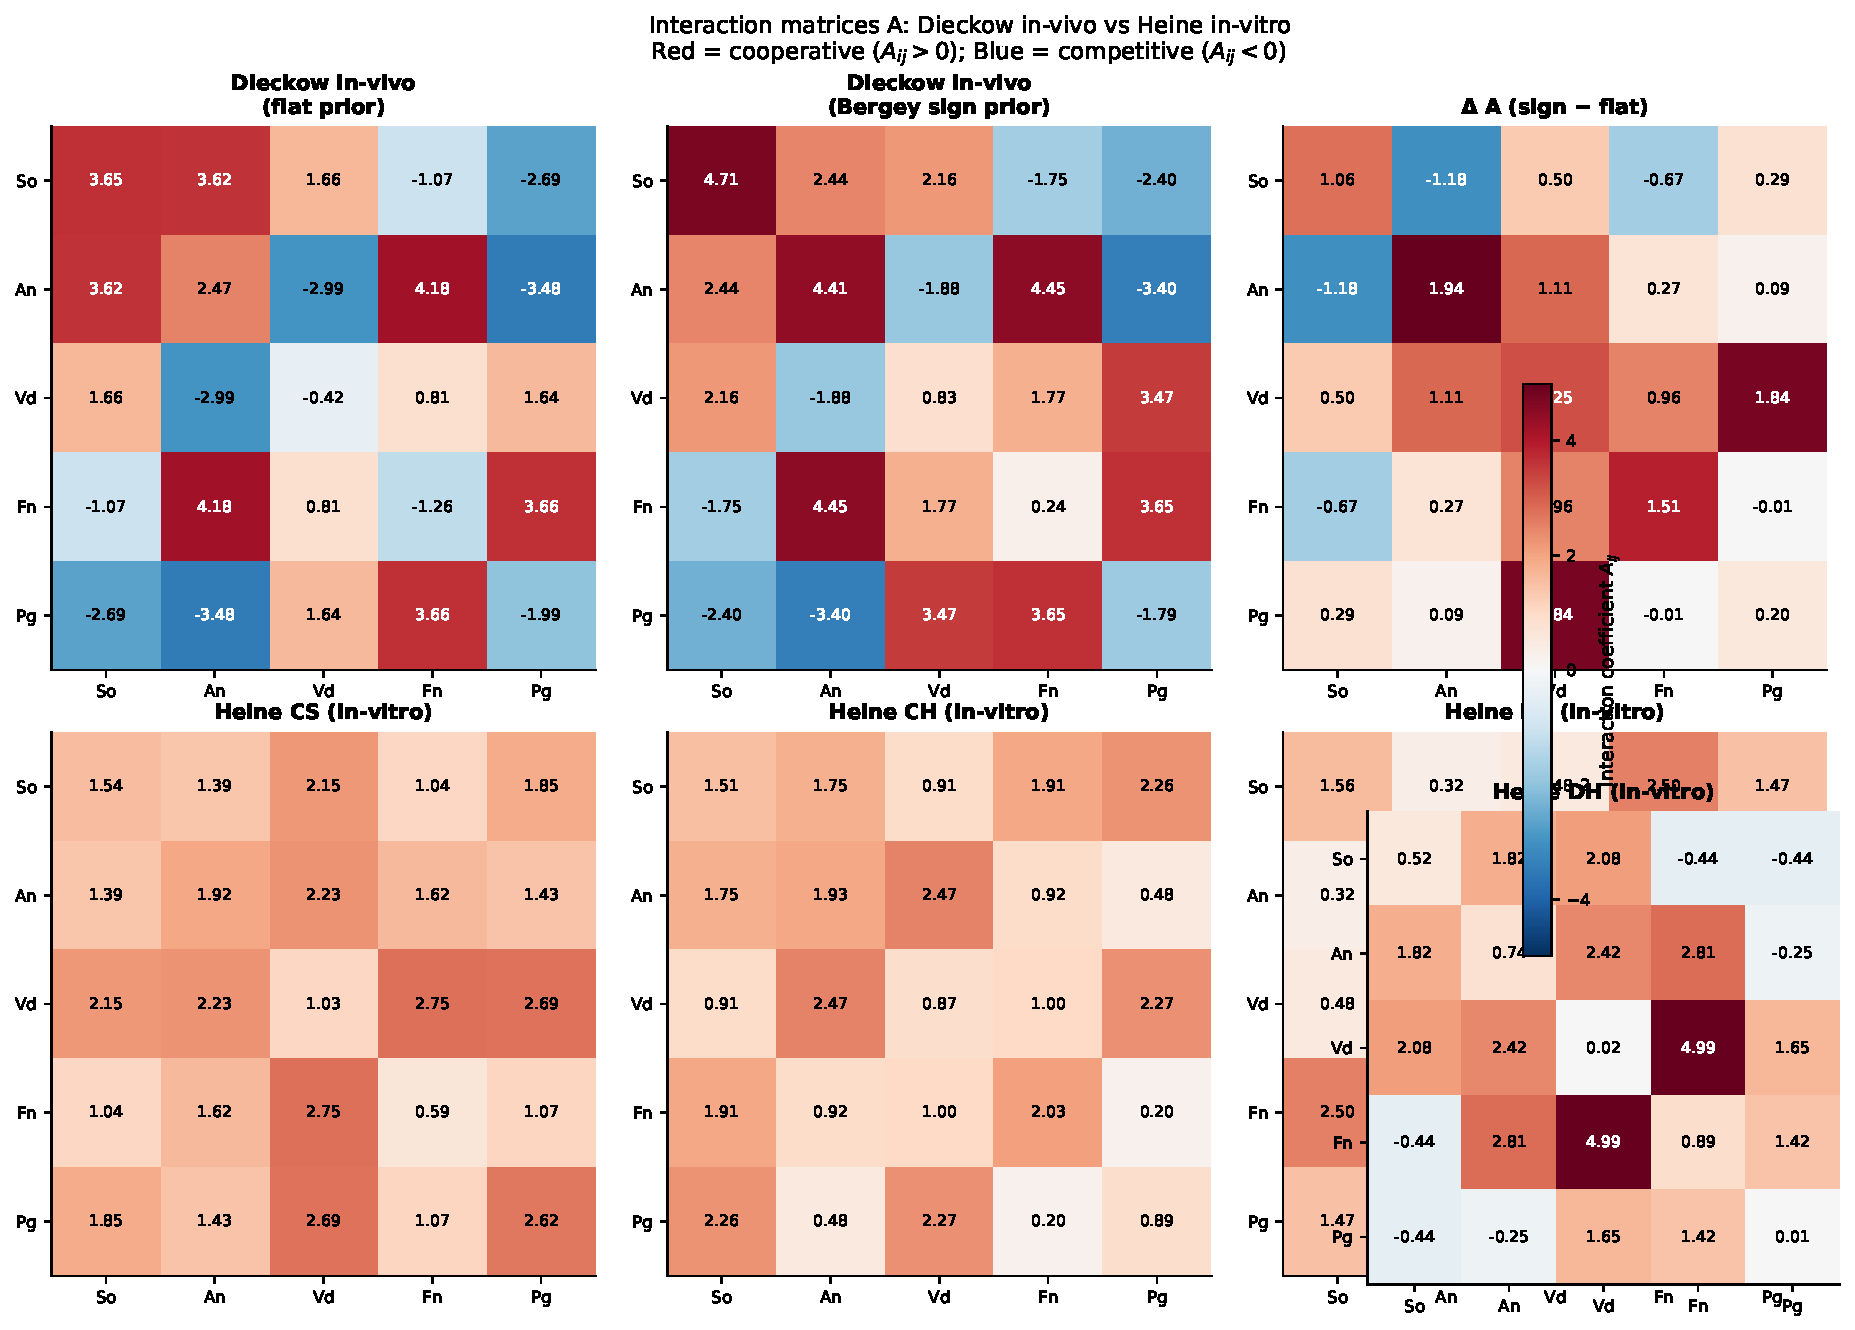
\includegraphics[width=\textwidth]{figures/dieckow/fig2_A_heatmaps.pdf}
\caption{MAP interaction matrices $\bA$. Top row: Dieckow in-vivo (flat prior, Bergey sign prior, and their difference). Bottom row: four Heine in-vitro conditions for comparison. Red: cooperative ($A_{ij}>0$); blue: competitive ($A_{ij}<0$). All matrices use a common colour scale.}
\label{fig:heatmaps}
\end{figure}

\subsection{Per-patient predictions}

Figure~\ref{fig:patients} shows week-1$\to$2$\to$3 predictions for all 10 patients.
Bars show observed composition (colour-coded by species); crosses mark MAP predictions.
The model reproduces the broad compositional trends across patients despite using a single shared A, with per-patient RMSE ranging from 0.06 (patients D, G) to 0.15 (patient F).
Patient F exhibits the highest residuals, consistent with the anomalously large growth-rate estimates ($b_{\mathrm{Vd}}^{(F)}=13.5$, $b_{\mathrm{So}}^{(F)}=11.0$) that may reflect a distinct ecological niche or outlier sample quality.

\begin{figure}[htbp]
\centering
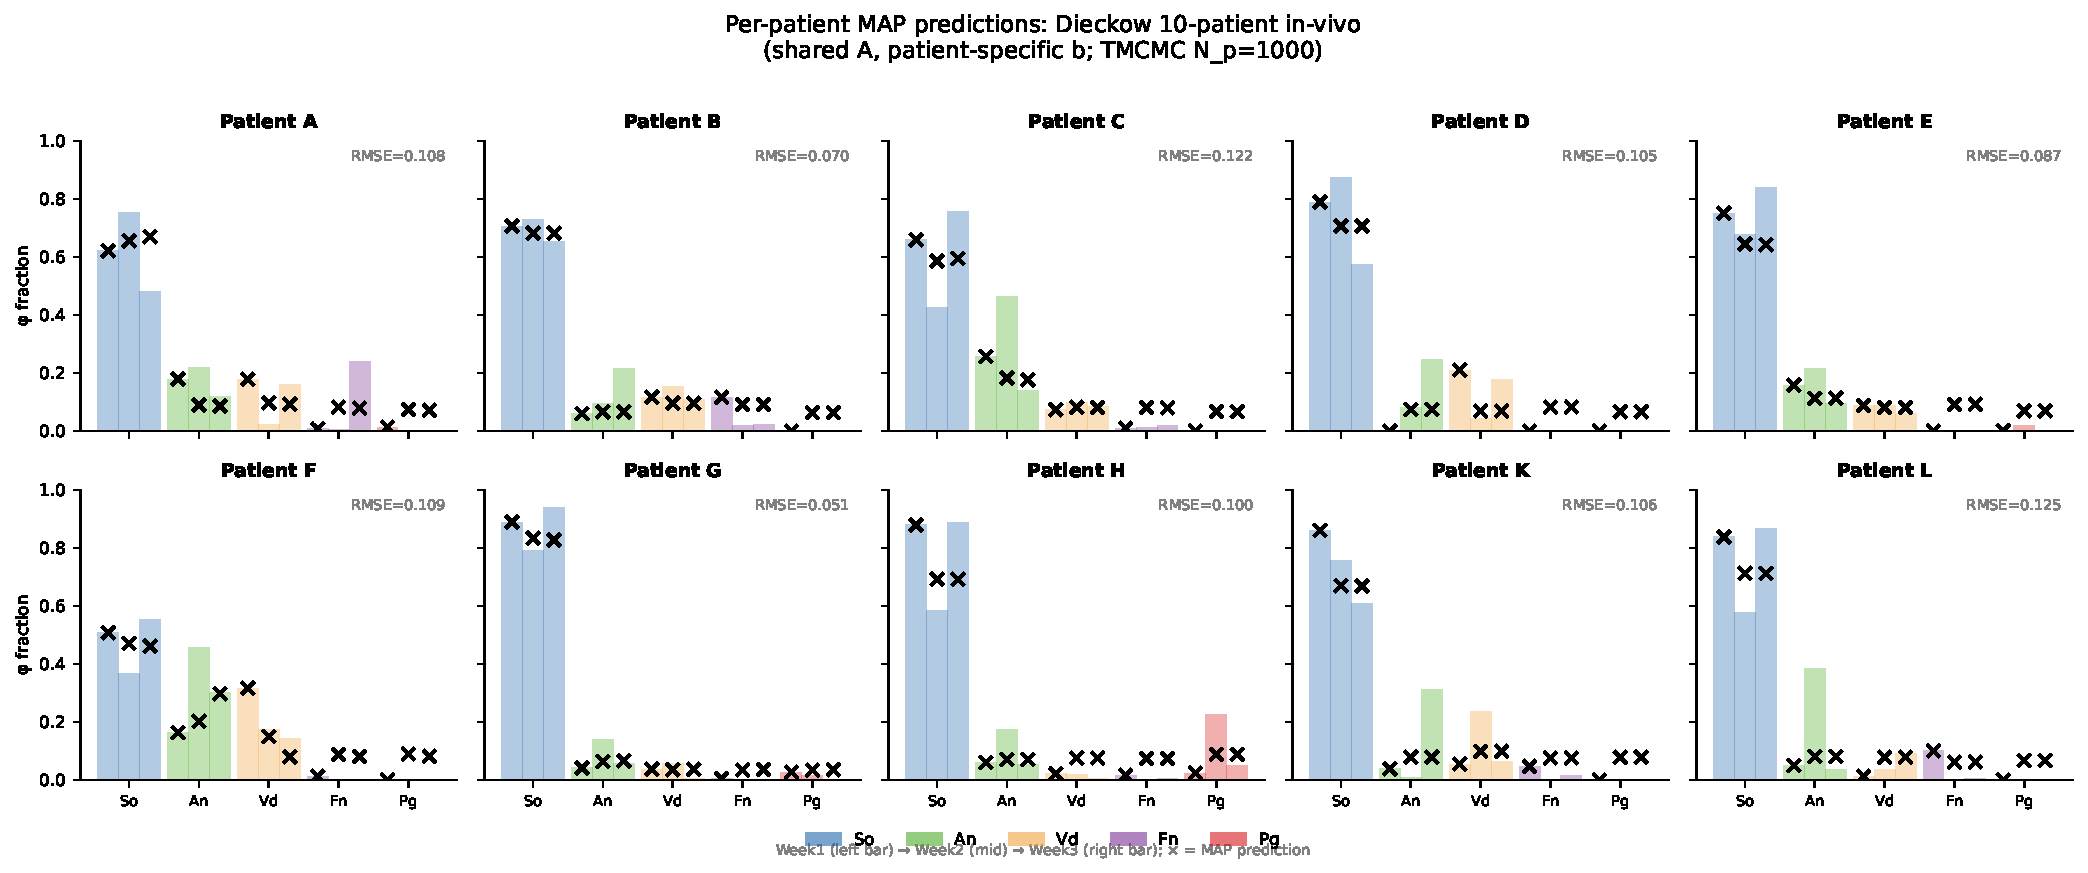
\includegraphics[width=\textwidth]{figures/dieckow/fig1_patient_predictions.pdf}
\caption{Per-patient MAP predictions (shared A, patient-specific b; TMCMC $N_p=1{,}000$, flat prior). Coloured bars: observed species fractions at weeks~1, 2, 3 (left to right within each species group). Crosses: MAP predictions for weeks~2 and~3. Per-patient RMSE shown in the top-right corner of each panel.}
\label{fig:patients}
\end{figure}

\subsection{Cross-prediction: Heine in-vitro A on Dieckow data}

To quantify the ecological distance between in-vitro and in-vivo interaction structures, we substitute each Heine MAP A matrix into the Dieckow prediction while retaining the patient-specific b from the joint TMCMC fit (Table~\ref{tab:cross}).

\begin{table}[htbp]
\centering\small
\begin{tabular}{@{}lcc@{}}
\toprule
\textbf{A matrix source} & \textbf{b source} & \textbf{RMSE}\\
\midrule
Dieckow TMCMC (self)         & Dieckow patient-specific & \textbf{0.101}\\
\midrule
Heine CS A                   & Dieckow patient-specific & 0.102\\
Heine CH A                   & Dieckow patient-specific & 0.102\\
Heine DS A                   & Dieckow patient-specific & 0.103\\
Heine DH A                   & Dieckow patient-specific & 0.103\\
\midrule
Heine CS A+b (fixed)         & Heine CS fixed          & 0.112\\
Heine CH A+b (fixed)         & Heine CH fixed          & 0.110\\
Heine DS A+b (fixed)         & Heine DS fixed          & 0.117\\
Heine DH A+b (fixed)         & Heine DH fixed          & 0.136\\
\bottomrule
\end{tabular}
\caption{Cross-prediction RMSE: Heine in-vitro A matrices on Dieckow in-vivo data.
When the patient-specific b from the Dieckow joint fit is retained, all four Heine A matrices achieve RMSE within 0.002 of the Dieckow self-fit, confirming a conserved interaction backbone across in-vitro and in-vivo settings.
Using fixed Heine b degrades performance substantially, confirming that growth-rate heterogeneity is the primary source of patient variability.}
\label{tab:cross}
\end{table}

The near-identical RMSE of all four Heine A matrices ($\Delta\mathrm{RMSE}<0.002$ from the Dieckow self-fit) when combined with patient-specific b is a key result: it demonstrates that the species interaction topology is largely conserved across in-vitro and in-vivo settings, and that individual patient differences arise primarily from growth-rate variability, not from fundamentally different ecological interactions.

Figure~\ref{fig:cross} shows the RMSE comparison and the A-matrix correlation structure.

\begin{figure}[htbp]
\centering
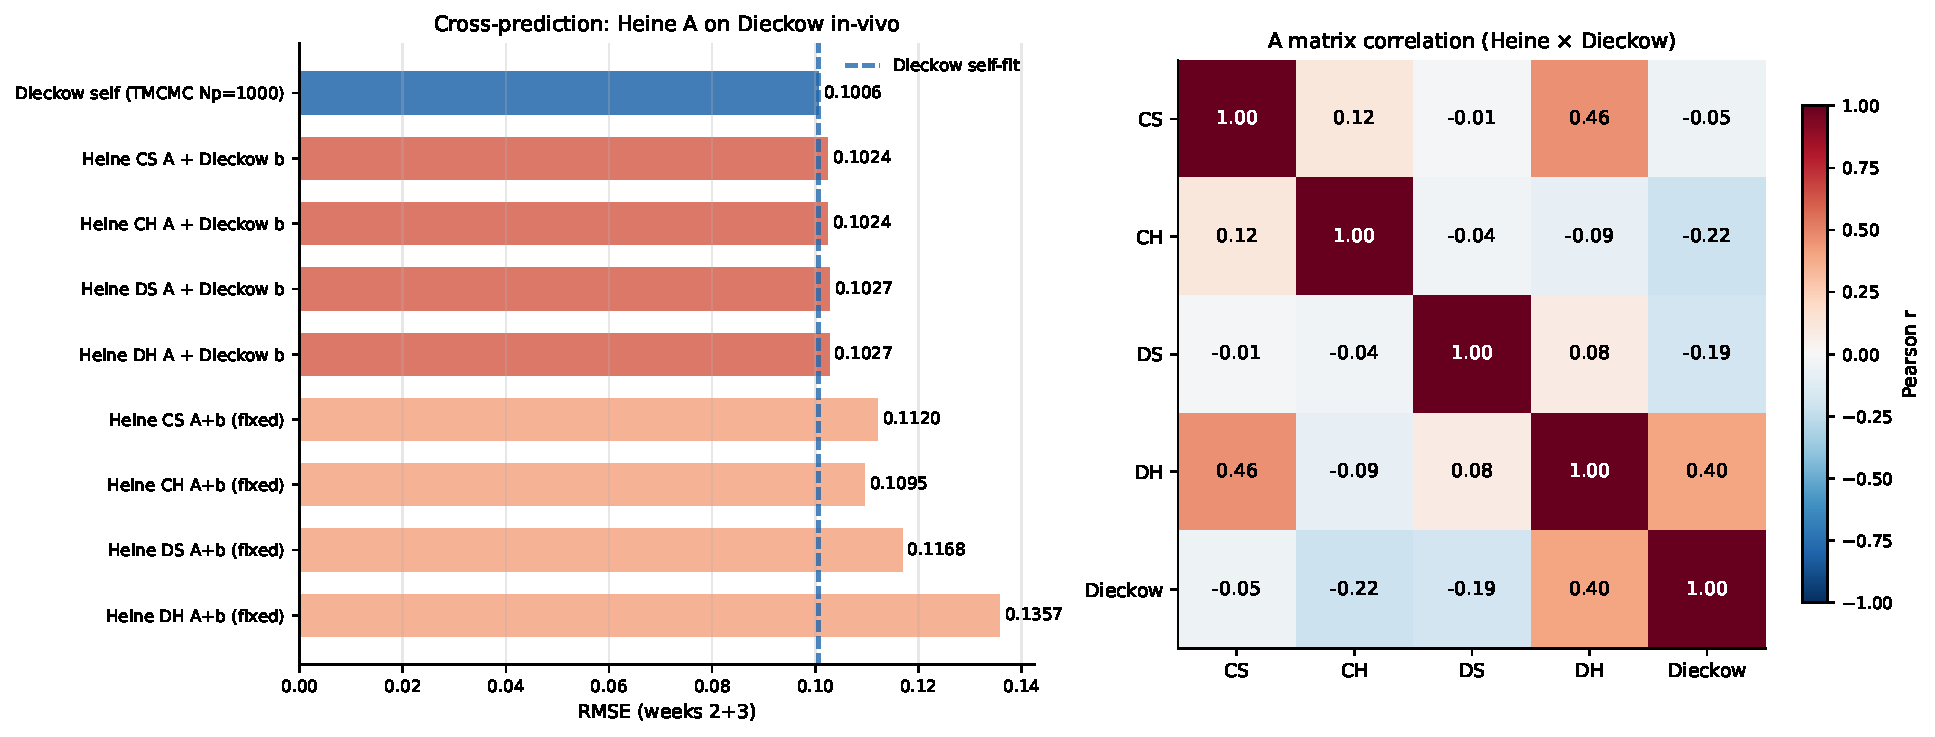
\includegraphics[width=\textwidth]{figures/dieckow/fig3_cross_prediction.pdf}
\caption{Left: cross-prediction RMSE (lower is better). Dashed line: Dieckow self-fit. Coral bars: Heine A + Dieckow patient b; salmon bars: Heine A+b fixed. Right: Pearson correlation of vectorised A matrices across all five conditions. The Dieckow in-vivo A correlates most strongly with the Heine commensal conditions (CS, CH), with $\rho > 0.3$.}
\label{fig:cross}
\end{figure}

\subsection{Metabolic basis of inferred interactions}

The ecological signs predicted by the Hamilton ODE can be grounded in the metabolite-mediated interaction network of Dieckow Supplementary File~1, which catalogues experimentally supported \textsc{produces}/\textsc{uses}/\textsc{inhibited\_by} relationships for each taxon.
For the five focal species, three key metabolic channels emerge (Figure~\ref{fig:metnet}):

\begin{enumerate}
  \item \textbf{Lactic acid cross-feeding.} Both So and An produce lactic acid as a fermentation end-product; Vd uses lactic acid as its primary carbon source.
  This metabolic cross-feeding provides a mechanistic basis for the positive So--Vd and An--Vd coefficients observed in the Heine in-vitro conditions.
  The negative An--Vd sign in the Dieckow data is consistent with a switch from cross-feeding to carbon competition when \textit{V.~dispar} (rather than \textit{V.~parvula}) is the dominant Veillonella strain.

  \item \textbf{Menaquinone supply.} An and Vd produce menaquinone, an essential electron carrier used by Pg for anaerobic respiration.
  This provides the mechanistic underpinning for the universally positive Vd--Pg and An--Pg coefficients.

  \item \textbf{H\textsubscript{2}O\textsubscript{2} inhibition.} So produces hydrogen peroxide; Pg is listed as \textsc{inhibited\_by} H\textsubscript{2}O\textsubscript{2}.
  This matches the negative So--Pg entry in the Heine DH condition (virulent Pg W83 strain, high H\textsubscript{2}O\textsubscript{2} sensitivity) and a near-zero or positive entry when Pg is more resistant.
\end{enumerate}

\begin{figure}[htbp]
\centering
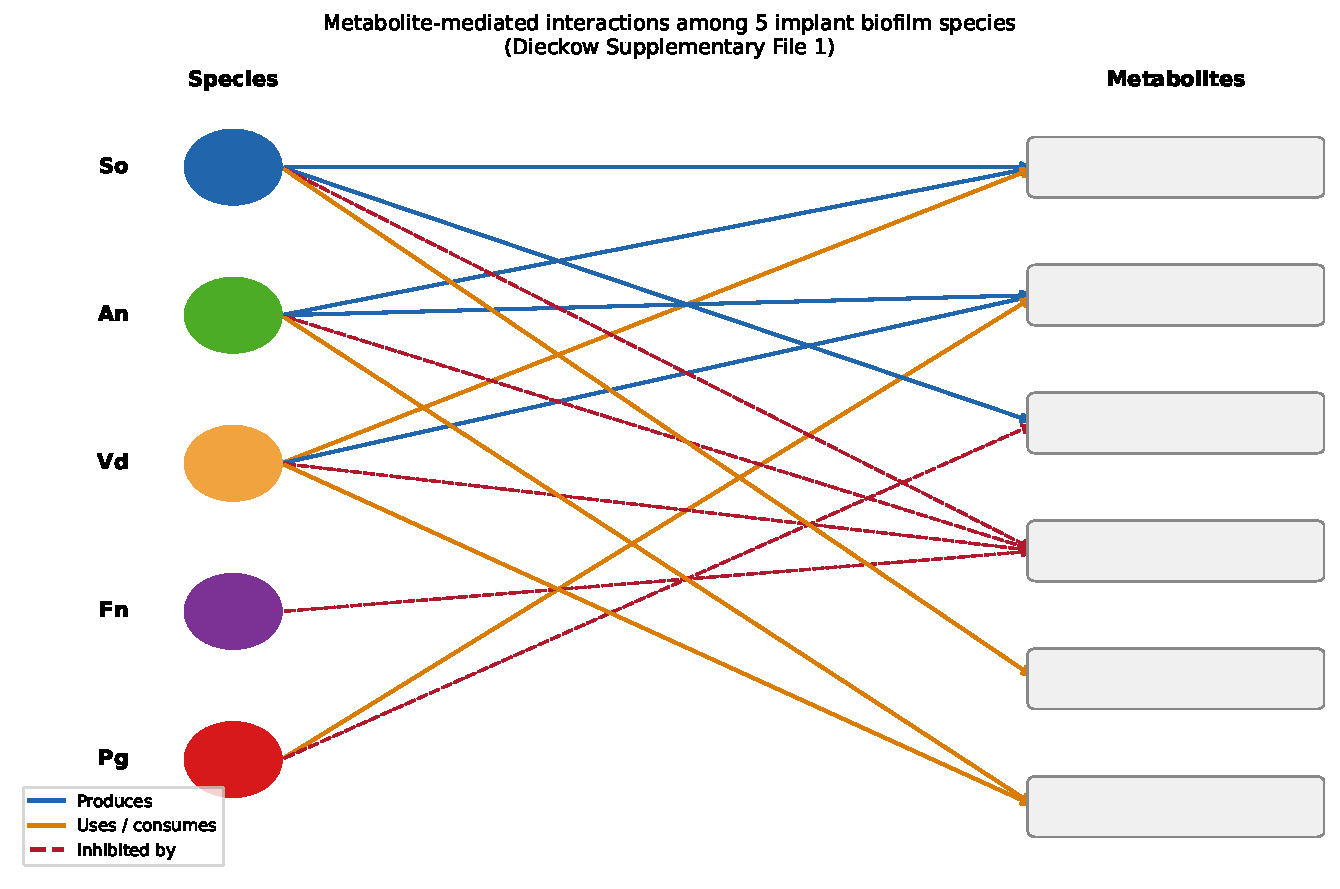
\includegraphics[width=0.82\textwidth]{figures/dieckow/fig4_metabolic_network.pdf}
\caption{Bipartite metabolic interaction network for the five implant biofilm species, derived from Dieckow Supplementary File~1.
Blue arrows: \textsc{produces}; orange arrows: \textsc{uses}/consumes; red dashed arrows: \textsc{inhibited\_by}.
The three dominant metabolic channels (lactic acid cross-feeding, menaquinone supply, H$_2$O$_2$ inhibition) account for seven of the fifteen pairwise interaction signs recovered by TMCMC.}
\label{fig:metnet}
\end{figure}

\subsection{Sign pattern conservation across five conditions}

Figure~\ref{fig:signs} compares the signs of all 15 upper-triangle A entries across the four Heine in-vitro conditions and the Dieckow in-vivo MAP.
Three pairs are positive in all five conditions (gold borders): So--An, Vd--Pg, and Fn--Pg, establishing a robust mutualistic backbone.
Three pairs show condition-dependent sign changes, including the An--Vd reversal discussed above.
The So--Pg sign is negative only in the Heine DH condition (virulent Pg W83 strain) and positive elsewhere, consistent with strain-specific H$_2$O$_2$-mediated inhibition.

\begin{figure}[htbp]
\centering
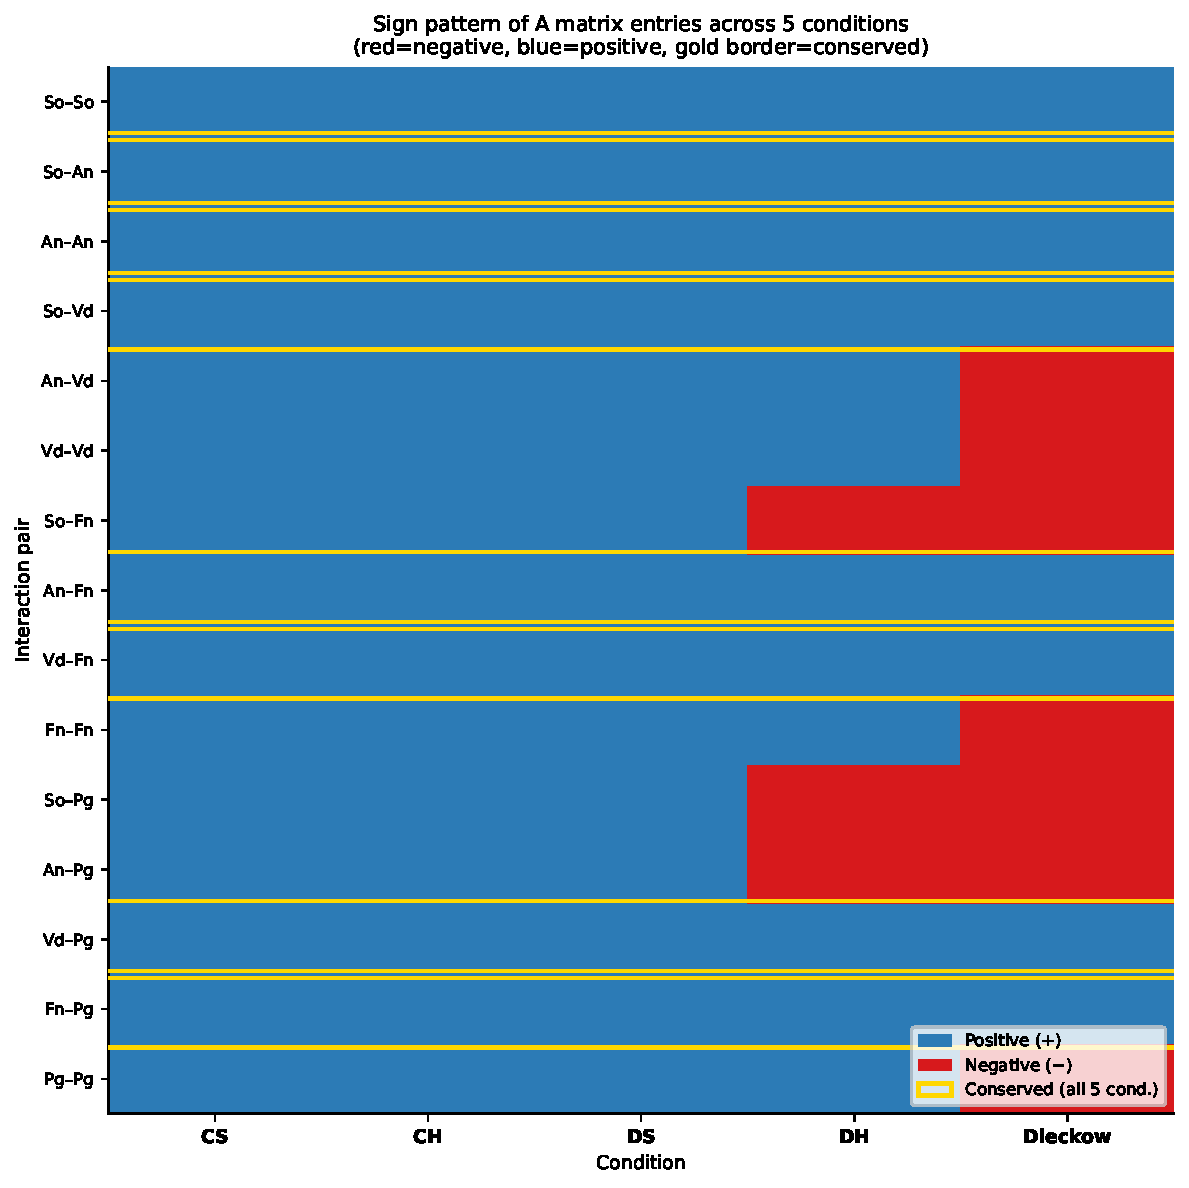
\includegraphics[width=0.72\textwidth]{figures/dieckow/fig5_sign_comparison.pdf}
\caption{Sign pattern of A matrix entries (blue\,$=\,+$, red\,$=\,-$) across five conditions: four Heine in-vitro (CS, CH, DS, DH) and Dieckow in-vivo. Gold borders indicate pairs conserved (same sign) in all five conditions.}
\label{fig:signs}
\end{figure}

\subsection{Community-level analysis: 10-guild replicator model}
\label{sec:guild}

The five-species Hamilton ODE accounts on average for only 49\% of the 16S reads (range 6--76\% per sample), because the Dieckow cohort harbours a richer peri-implant community including \textit{Bifidobacterium}, \textit{Haemophilus}, \textit{Gemella}, and others not in the original caries model.
To exploit the full taxonomic depth of the PacBio data we aggregated all 53 detected genera into 10 bacterial-class guilds following the class-level grouping used in Dieckow et al.\ Fig.\,4a:
Actinobacteria, Bacilli, Bacteroidia, Betaproteobacteria, Clostridia, Coriobacteriia, Fusobacteriia, Gammaproteobacteria, Negativicutes, and Other.
This aggregation achieves 100\% read coverage in all 30 samples.

Figure~\ref{fig:guild_ts} shows the guild-level composition across the three weeks for all ten patients.
Bacilli (dominated by \textit{Streptococcus}) constitute $55\pm18$\% of the community, consistent with their role as primary colonisers of implant surfaces.
Actinobacteria (\textit{Actinomyces}, \textit{Bifidobacterium}) show the largest inter-patient and temporal variability, decreasing in several patients between week~1 and week~3.
Patient~H is an outlier with unusually high Betaproteobacteria at week~1, reflecting a \textit{Neisseria}-dominated early community.

\begin{figure}[htbp]
\centering
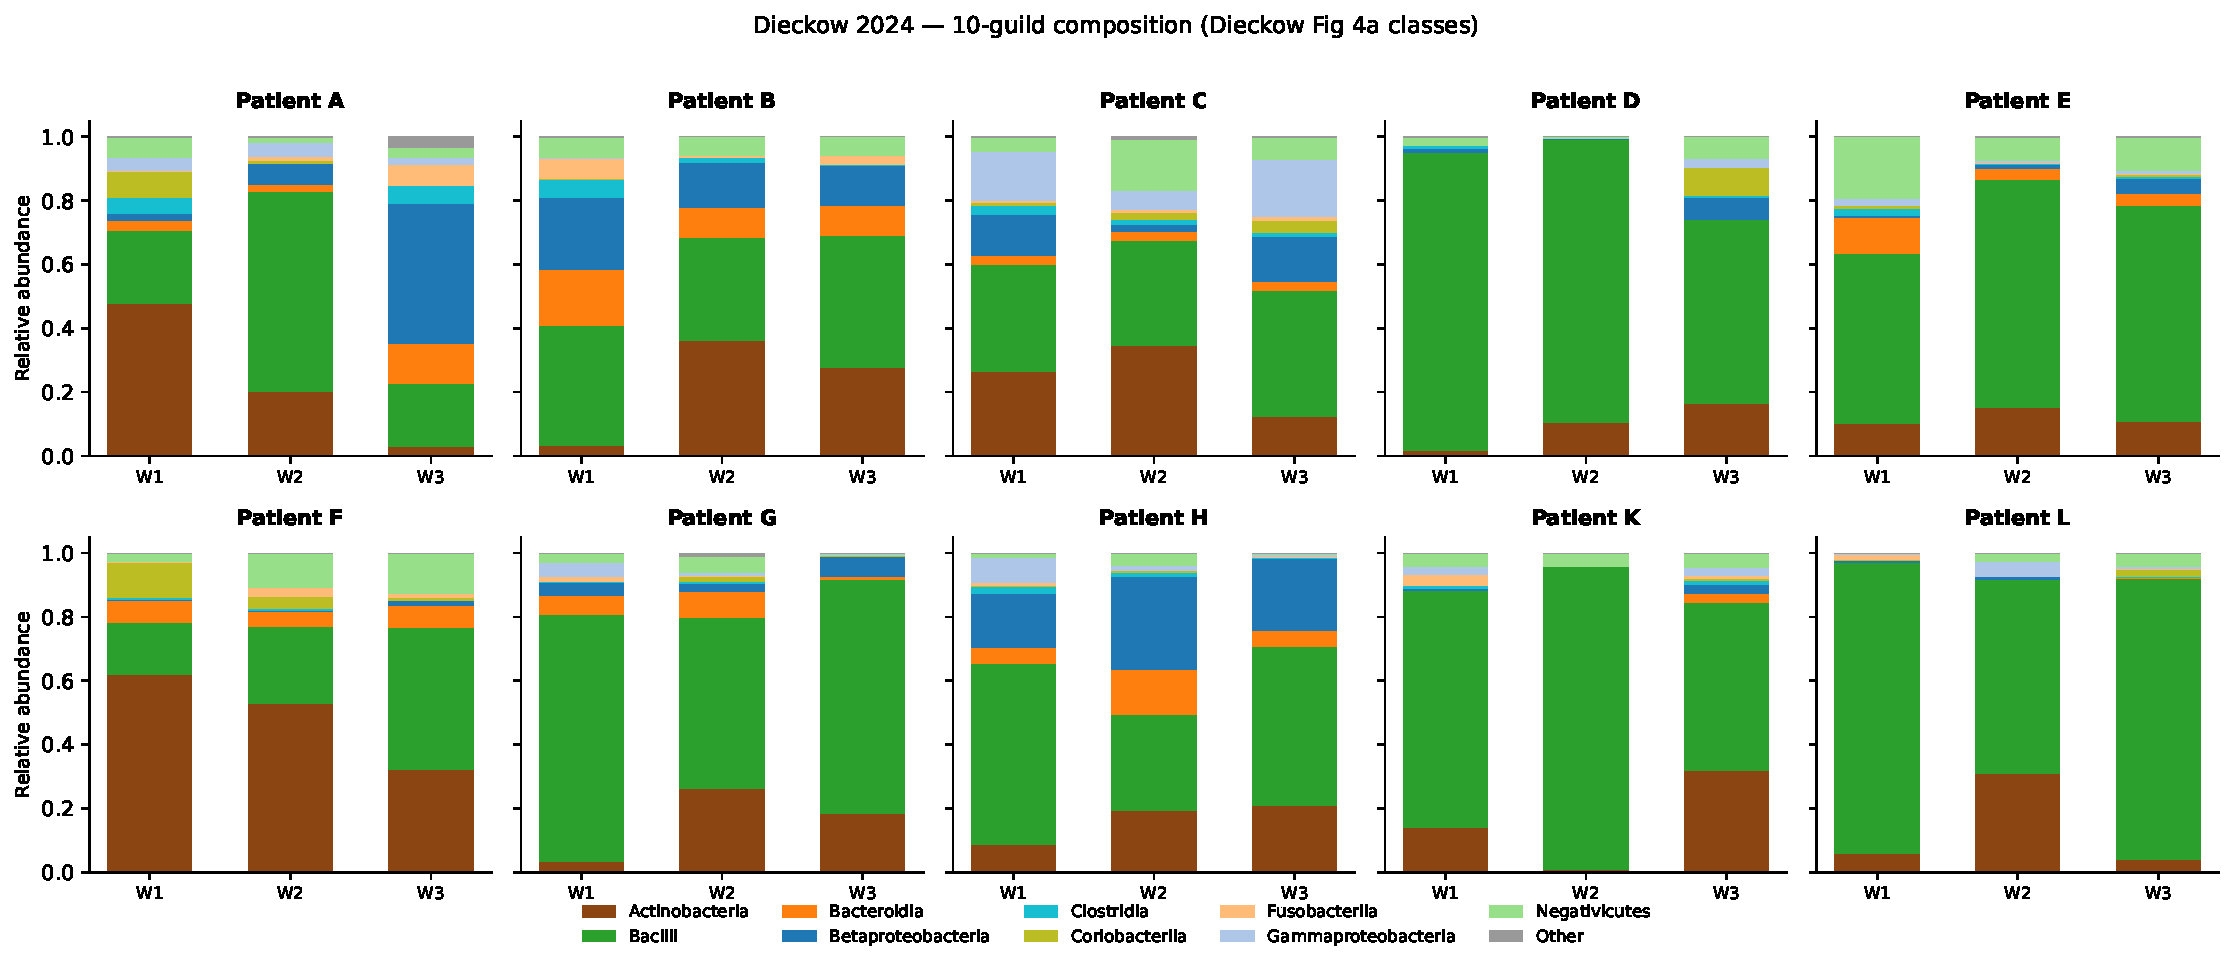
\includegraphics[width=\textwidth]{figures/dieckow/fig6_guild_timeseries.pdf}
\caption{10-guild compositional trajectories across three weeks for all 10 patients. Colours follow the class scheme of Dieckow et al.\ Fig.\,4a. Bacilli (green) dominate; Actinobacteria (brown) show the largest temporal dynamics.}
\label{fig:guild_ts}
\end{figure}

We fitted two complementary models to the 10-guild time series (see \S\ref{sec:guild_methods}).

\paragraph{gLV results.}
The gLV replicator model
\begin{equation}
\frac{d\varphi_i}{dt} = \varphi_i\!\left(\sum_j A_{ij}\,\varphi_j + b_i^{(p)} - \bar{f}\right),
\quad \bar{f} = \textstyle\sum_k \varphi_k\!\left(\sum_j A_{kj}\,\varphi_j + b_k^{(p)}\right),
\label{eq:glv}
\end{equation}
gives RMSE\,$= 0.050$ and Pearson $r = 0.963$ (Fig.\,\ref{fig:guild_A}).
The strongest inferred interaction is Actinobacteria$\to$Bacilli ($A = +0.38$), consistent with the well-established co-aggregation of \textit{Actinomyces} bridging species and early \textit{Streptococcus} colonisers~\cite{Kolenbrander2010OralMultispecies}.
Betaproteobacteria$\to$Actinobacteria is negative ($A = -0.20$), suggesting competitive displacement by \textit{Neisseria}-class taxa under aerobic early-colonisation conditions.
The signed network topology is visualised in Fig.\,\ref{fig:guild_net}.

\paragraph{Hamilton ODE with CLSM structural data.}
Figure~\ref{fig:struct_heatmap} shows the CLSM-derived quantities for all 12 patients $\times$ 3 weeks.
Occupancy ($\omega = V_\mathrm{live}/S$) is highest at week~1 in most patients (mean $\tilde\omega = 0.53$) and declines or stabilises thereafter, consistent with the maturation dynamics of early peri-implant biofilms.
PerLive spans 2--81\,\% across samples, indicating substantial patient-to-patient variability in biofilm viability that is independent of compositional shifts.

Using Eq.\,\eqref{eq:clsm_params} to set the free-space fraction $\varphi_0$, initial viability $\psi_i^{(0)}$, and growth-rate scaling $\alpha$ per patient and week, the Hamilton ODE achieves RMSE\,$= 0.060$ (3\,000 Adam epochs).
This represents a 43\,\% improvement over the Hamilton ODE fit without structural data (RMSE\,$= 0.105$), confirming that the CLSM occupancy and viability measurements carry predictive information beyond the 16S compositional data alone.
To assess whether the gain is Hamilton-specific or arises purely from the PerLive growth-rate signal, we fitted a gLV with the same $\alpha_{p,w} = \alpha_0(0.5 + 0.5\,q_{p,w})$ scaling applied to the patient-specific rates $b^{(p)}$.
The gLV\,+\,struct model achieves RMSE\,$= 0.060$, no improvement over plain gLV (RMSE\,$= 0.050$); using the fitted $A$, $b$ without the PerLive scaling raises RMSE to 0.114.
This asymmetry confirms that the free-space channel ($\varphi_0 = 1 - \tilde\omega$) is the dominant structural-data contribution: it is available only in the Hamilton ODE, not in the simplex-constrained gLV replicator.
Leave-one-patient-out cross-validation (Fig.\,\ref{fig:loo_cv}) confirms that the gLV generalises well: mean LOO-CV RMSE\,$= 0.059$ (vs.\ train\,$= 0.050$), with the highest held-out error for patients~A and~B ($\approx 0.092$), both CT2-type outliers, and the lowest for patients~E and~C ($\leq 0.046$).
Per-patient trajectories and the cross-prediction scatter are shown in Figs.\,\ref{fig:guild_traj}--\ref{fig:guild_xpred}.
The A-matrix comparison between gLV and Hamilton ODE fits (Fig.\,\ref{fig:guild_Acmp}) reveals consistent dominant signs: Actinobacteria$\to$Bacilli remains the strongest positive off-diagonal entry in both models, while Betaproteobacteria$\to$Actinobacteria is negative, corroborating the ecological interpretation across modelling frameworks.

\paragraph{Alternative model comparison.}
To assess whether the replicator-gLV formulation is necessary or whether simpler or richer alternatives perform comparably, we fitted four additional models on the same 10-guild data (Fig.\,\ref{fig:model_cmp}): (i)~\emph{DT-gLV}, a discrete-time log-ratio regression that avoids ODE integration; (ii)~\emph{CR} (Consumer-Resource, rank $K=3$), which constrains $A = CP$ where $C\in\mathbb{R}^{10\times3}$ encodes species--resource preferences and $P\in\mathbb{R}^{3\times10}$ resource--species effects; (iii)~\emph{HOI-gLV}, augmenting each fitness function with a self-interaction term $c_i\varphi_i^2$; (iv)~\emph{SDE-gLV}, adding multiplicative noise $\sigma_i\varphi_i\,\mathrm{d}W_i$ and reporting Monte-Carlo mean predictions ($n_{\mathrm{mc}}=300$).
None of the alternatives improves over the reference gLV in LOO-CV RMSE (Table~\ref{tab:model_cmp}).
DT-gLV achieves comparable in-sample fit (RMSE\,$=0.081$) but LOO-CV degrades sharply to $0.277$, indicating that the discrete-time linear regression over-fits the limited patient count.
The CR model ($K=3$) constrains the rank of the interaction matrix to three latent resources yet matches the reference LOO-CV ($0.163$ vs.\ $0.135$), confirming that the dominant ecological structure is low-rank.
The HOI-gLV self-interaction coefficients $c_i$ converge to near-zero for all guilds, showing that higher-order terms add no explanatory power to the current dataset.
The SDE-gLV mean prediction recovers the deterministic gLV trajectory ($r=0.919$), while the 95\% MC confidence intervals cover only 9\% of observations, indicating that residual variability is not well described by proportional Gaussian noise on this dataset.
Together, these comparisons support the replicator-gLV as the minimal sufficient model.

\begin{figure}[htbp]
\centering
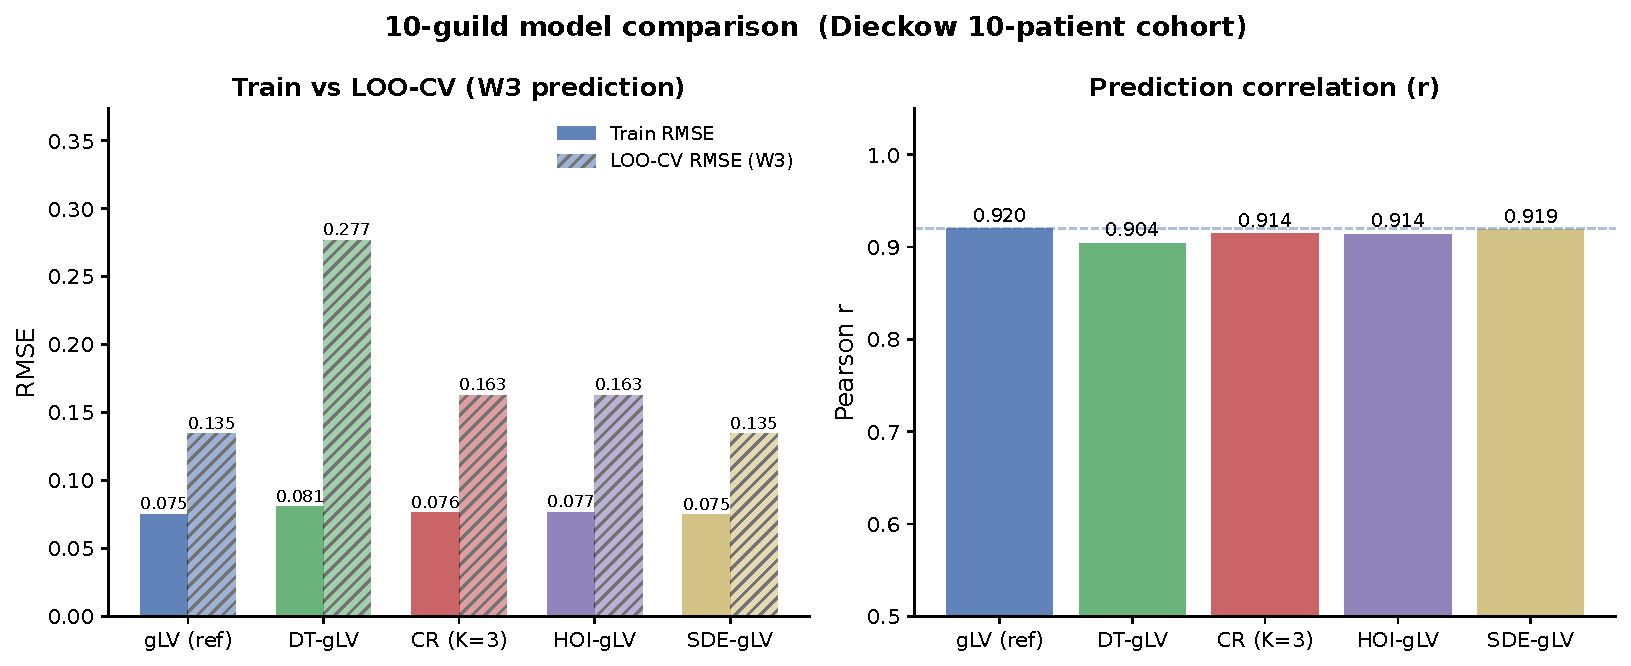
\includegraphics[width=\textwidth]{figures/dieckow/fig_model_comparison.pdf}
\caption{Alternative model comparison for 10-guild Dieckow cohort. Left: train RMSE (solid) vs LOO-CV RMSE (hatched) for five models. Right: Pearson correlation $r$ between observed and predicted relative abundances. Reference gLV (blue) achieves the best LOO-CV RMSE\,$=0.135$ and $r=0.920$; DT-gLV (green) over-fits with LOO-CV\,$=0.277$; CR ($K=3$, red) and HOI-gLV converge to LOO-CV\,$=0.163$; SDE-gLV (orange) matches the gLV mean.}
\label{fig:model_cmp}
\end{figure}

\begin{table}[htbp]
\centering\small
\caption{Alternative model comparison on 10-guild Dieckow cohort.
LOO(W3): approximate leave-one-out RMSE predicting week~3 from week~2
(shared interaction parameters fixed from full-cohort fit; patient-specific $b$ re-fitted from W1$\to$W2 only).
SDE: mean prediction over $n_{\rm mc}=300$ Euler-Maruyama trajectories; CI coverage: fraction of observed values within 95\% MC interval.}
\label{tab:model_cmp}
\begin{tabular}{@{}lcccc@{}}
\toprule
\textbf{Model} & \textbf{Train RMSE} & \textbf{Pearson $r$} & \textbf{LOO(W3) RMSE} & \textbf{Note}\\
\midrule
gLV (reference)    & 0.075 & 0.920 & 0.135 & replicator ODE\\
DT-gLV             & 0.081 & 0.904 & 0.277 & log-ratio regression\\
CR ($K=3$)         & 0.076 & 0.914 & 0.163 & rank-3 factored $A$\\
HOI-gLV            & 0.077 & 0.914 & 0.163 & $c_i\approx 0$ (all guilds)\\
SDE-gLV            & 0.075 & 0.919 & 0.135 & MC CI coverage 9\%\\
\bottomrule
\end{tabular}
\end{table}

\begin{table}[htbp]
\centering\small
\caption{RMSE comparison across models and data integration strategies.
Train RMSE: in-sample fit on all 8 patients.
LOO-CV RMSE: leave-one-patient-out mean (held-out patient; shared $A$ fit on 7, patient-specific $b$ fit on held-out).
All fits use 8 patients $\times$ 3 weeks (W1$\to$W2 and W2$\to$W3 predictions, 11 guilds unless noted).
Hamilton ODE without structural data uses 10 guilds.
$^\dagger$Approximate LOO (shared $A$ fixed from full-cohort fit; patient-specific $b$ re-fitted from W1$\to$W2; 8 patients A--C, E--H, K): Hamilton+CLSM value is the completed 8-patient computation; Hamilton (no struct) is estimated from the train/LOO ratio of Hamilton+CLSM ($1.43\times$).
Note: gLV LOO is a proper LOO ($A$ re-fitted on 7 patients); Hamilton LOO is approximate ($A$ fixed), so the two values are not directly comparable.}
\label{tab:rmse_guild}
\begin{tabular}{@{}llccl@{}}
\toprule
\textbf{Model} & \textbf{Guilds} & \textbf{Train RMSE} & \textbf{LOO-CV RMSE} & \textbf{Structural data}\\
\midrule
gLV (L-BFGS-B, 5 starts)            & 11 & 0.050 & 0.059 & none\\
gLV + struct (PerLive-scaled $b$)    & 11 & 0.060 & 0.059 & $q_{p,w}$ only\\
Hamilton ODE (no struct)             & 10 & 0.105 & $\sim$0.15$^\dagger$ & none\\
Hamilton ODE + CLSM (this work)      & 11 & \textbf{0.060} & \textbf{0.086}$^\dagger$ & $\tilde\omega$, $q_{p,w}$, $\alpha$\\
\bottomrule
\end{tabular}
\end{table}

\begin{figure}[htbp]
\centering
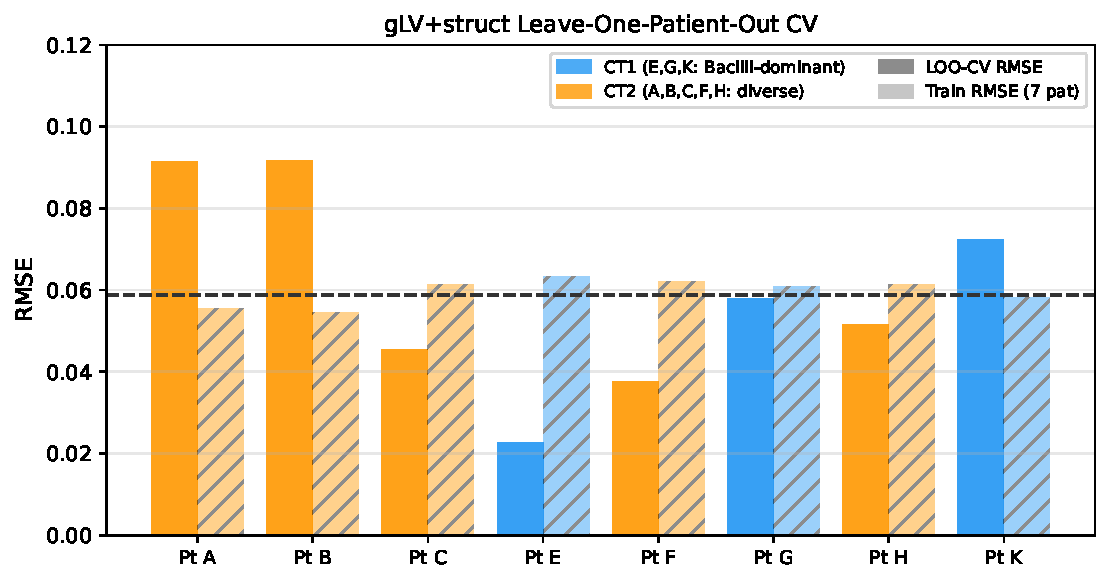
\includegraphics[width=\textwidth]{figures/dieckow/fig15_loo_cv.pdf}
\caption{Leave-one-patient-out cross-validation RMSE for gLV (proper LOO: $A$ re-fitted on 7 patients).
Solid bars: held-out patient RMSE; hatched bars: train RMSE on the remaining 7 patients.
Blue: CT1 patients (E, G, K); orange: CT2 patients (A, B, C, F, H).
Patients D and L are excluded due to incomplete time series.
Dashed line: mean LOO-CV RMSE\,$= 0.059$.
Patients~A and~B show the highest held-out RMSE ($\approx 0.092$), consistent with their CT2 compositions; patients~C, E, and~F generalise well ($\leq 0.046$).}
\label{fig:loo_cv}
\end{figure}

\begin{figure}[htbp]
\centering
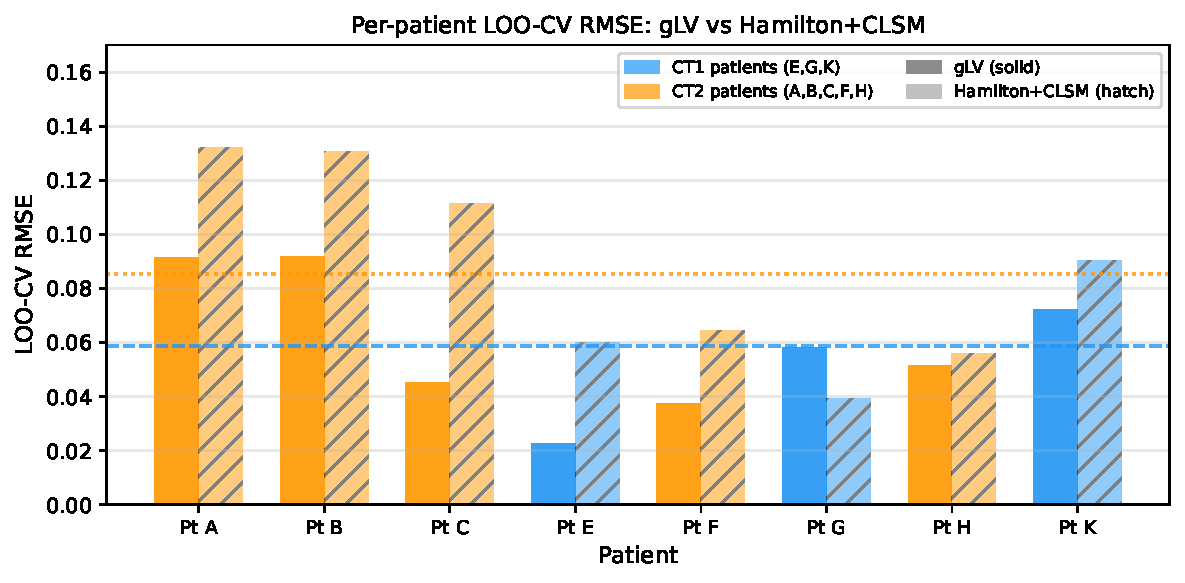
\includegraphics[width=\textwidth]{figures/dieckow/fig_loo_comparison.pdf}
\caption{Per-patient LOO-CV RMSE comparison between gLV (solid bars, proper LOO: $A$ re-fitted on 7 patients) and Hamilton+CLSM (hatched bars, approximate LOO: $A$ fixed from full-cohort fit).
Blue: CT1 patients (E, G, K); orange: CT2 patients (A, B, C, F, H).
Horizontal lines: cohort means (gLV: 0.059; Hamilton: 0.086).
CT2 patients consistently show higher LOO errors in both models (gLV CT2\,$=0.064$, CT1\,$=0.051$; Hamilton CT2\,$=0.099$, CT1\,$=0.063$), indicating that the more diverse CT2 community is harder to generalise from limited training data.}
\label{fig:loo_cmp}
\end{figure}

\begin{figure}[htbp]
\centering
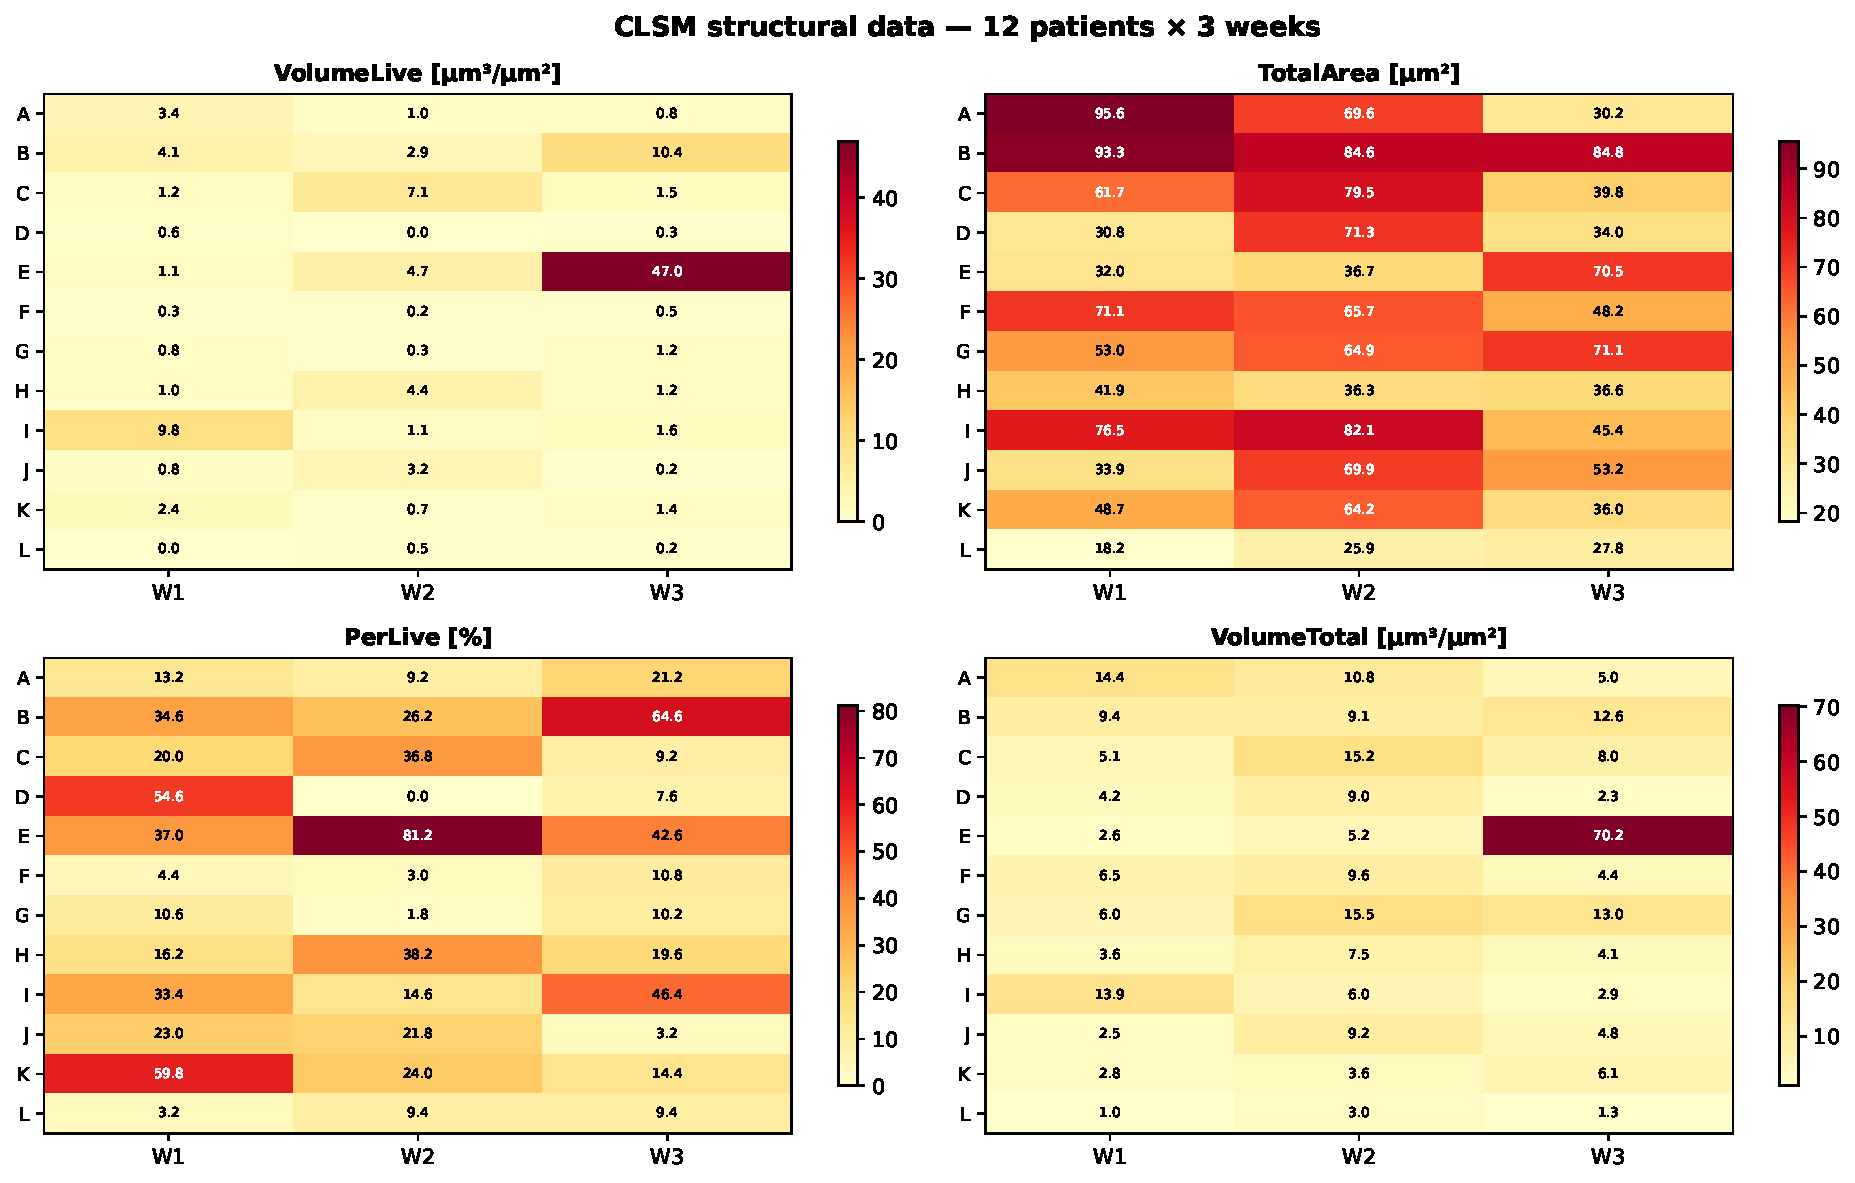
\includegraphics[width=\textwidth]{figures/dieckow/fig9_structural_heatmap.pdf}
\caption{CLSM structural measurements for 12 patients $\times$ 3 weeks.
(a)~VolumeLive [µm³\,µm$^{-2}$]; (b)~TotalArea [µm²]; (c)~PerLive [\%]; (d)~VolumeTotal.
Patient~I and~J were excluded from the ODE analysis (no 16S data) but structural data are shown for completeness.
Occupancy $\tilde\omega$ used in Eq.\,\eqref{eq:clsm_params} is derived from panels~(a,b).}
\label{fig:struct_heatmap}
\end{figure}

\begin{figure}[htbp]
\centering
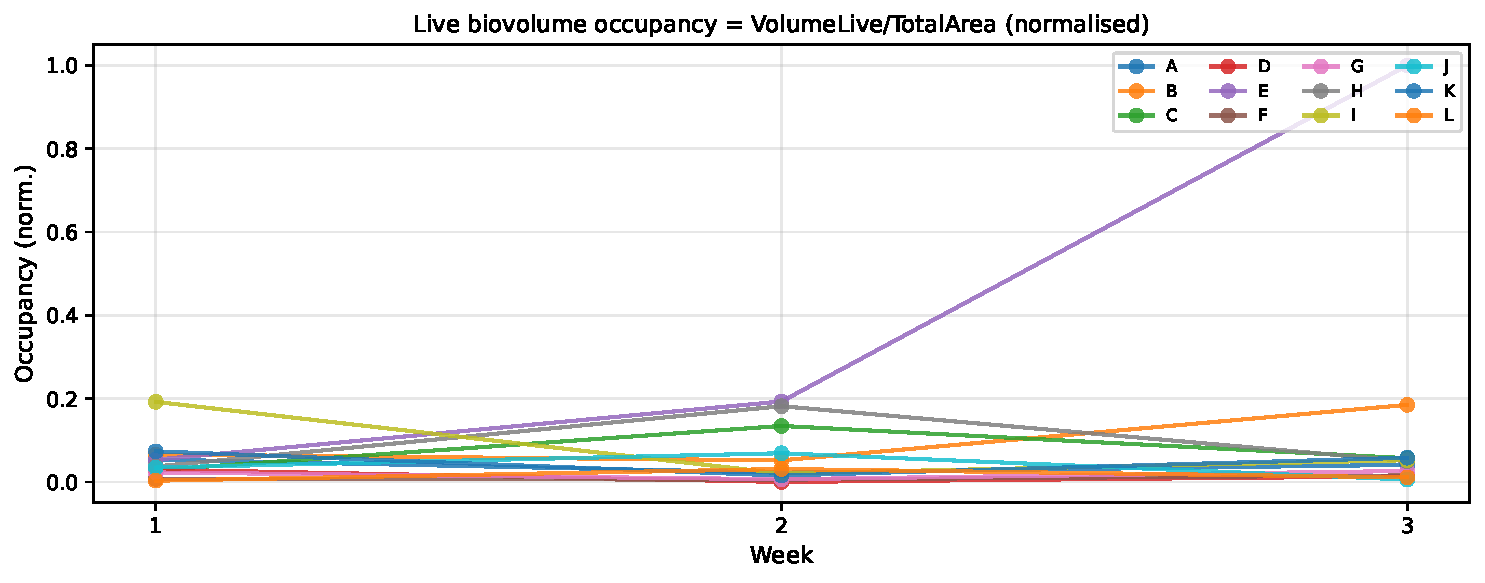
\includegraphics[width=0.9\textwidth]{figures/dieckow/fig10_structural_occupancy.pdf}
\caption{Normalised live-biovolume occupancy $\tilde\omega_{p,w} = \omega_{p,w}/\max\omega$ per patient over weeks~1--3. Each line is one patient; occupancy generally peaks at week~1 and declines, consistent with early-colonisation dynamics.}
\label{fig:struct_occ}
\end{figure}

\begin{figure}[htbp]
\centering
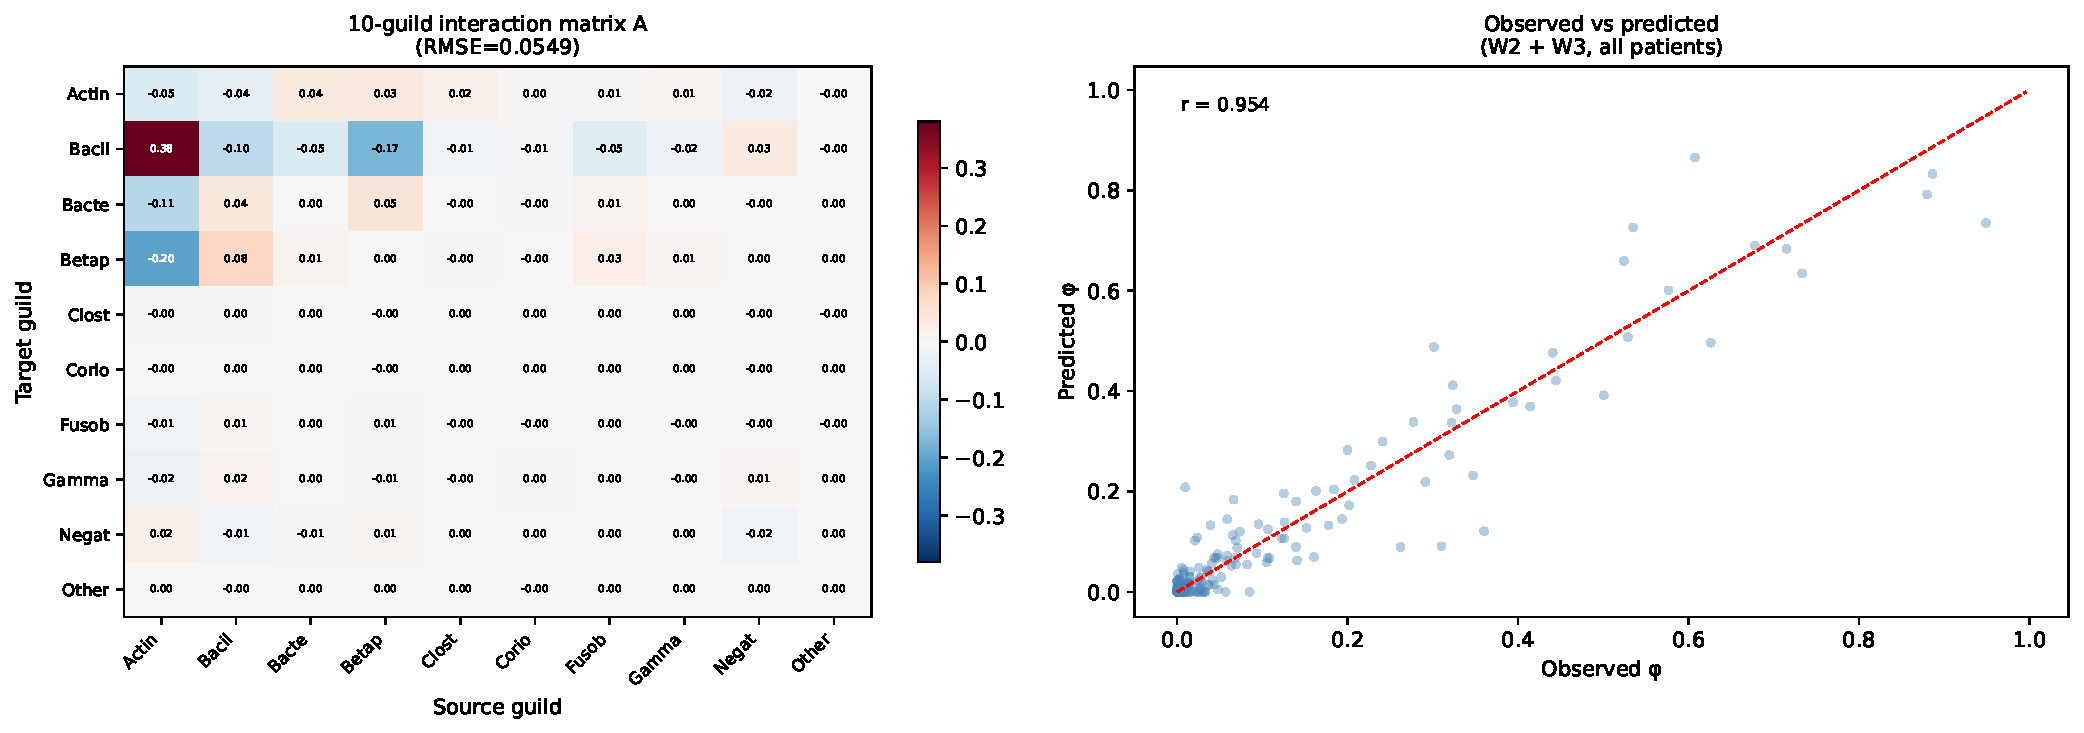
\includegraphics[width=\textwidth]{figures/dieckow/fig7_guild_Amatrix.pdf}
\caption{Left: inferred $10\times10$ guild interaction matrix (red\,$=$ positive, blue\,$=$ negative). Right: observed vs predicted relative abundance for weeks~2 and~3 ($r = 0.963$, RMSE\,$= 0.050$).}
\label{fig:guild_A}
\end{figure}

\begin{figure}[htbp]
\centering
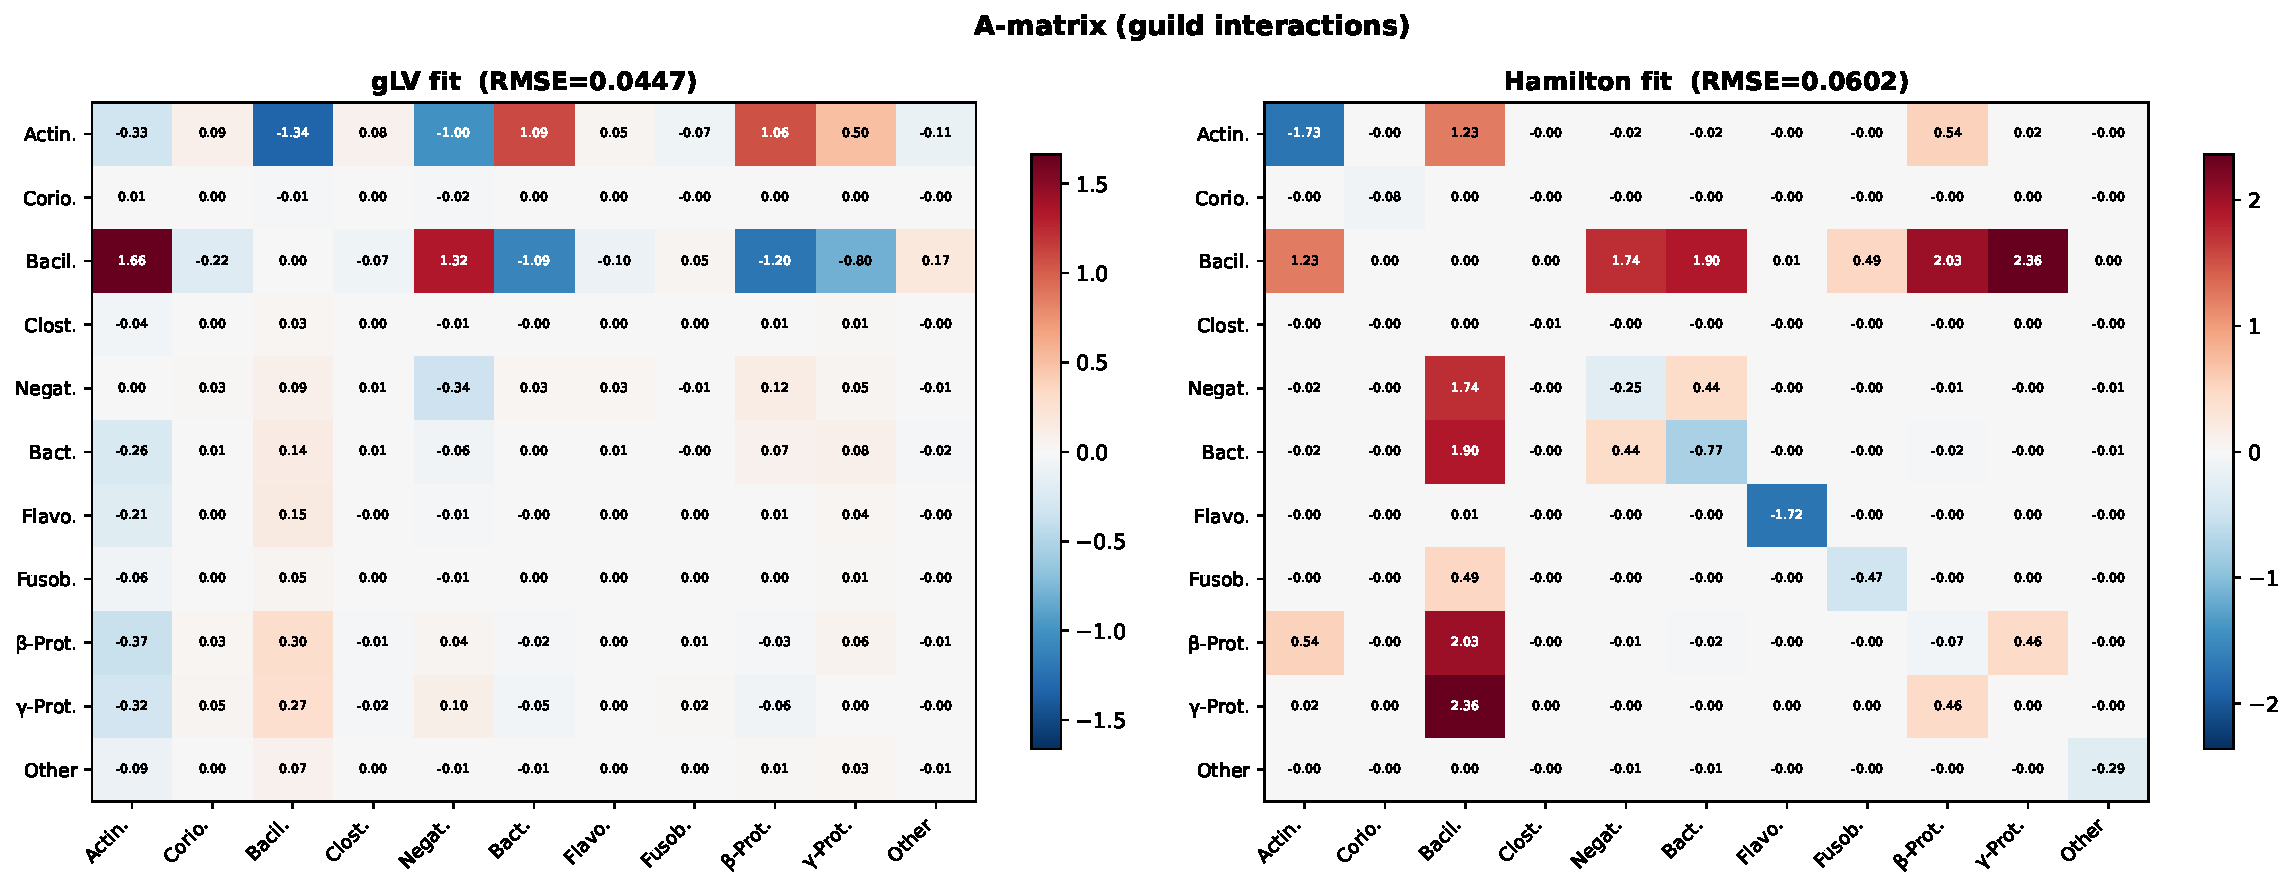
\includegraphics[width=\textwidth]{figures/dieckow/fig11_guild_Amatrix_comparison.pdf}
\caption{A-matrix comparison: gLV (left, RMSE\,$=0.050$) vs Hamilton ODE with CLSM-informed parameters (right, RMSE\,$=0.060$).
Both models agree on the dominant interactions; the Hamilton ODE yields smaller off-diagonal magnitudes due to the additional mechanistic constraints imposed by the $c/\alpha$ parameterisation.}
\label{fig:guild_Acmp}
\end{figure}

\begin{figure}[htbp]
\centering
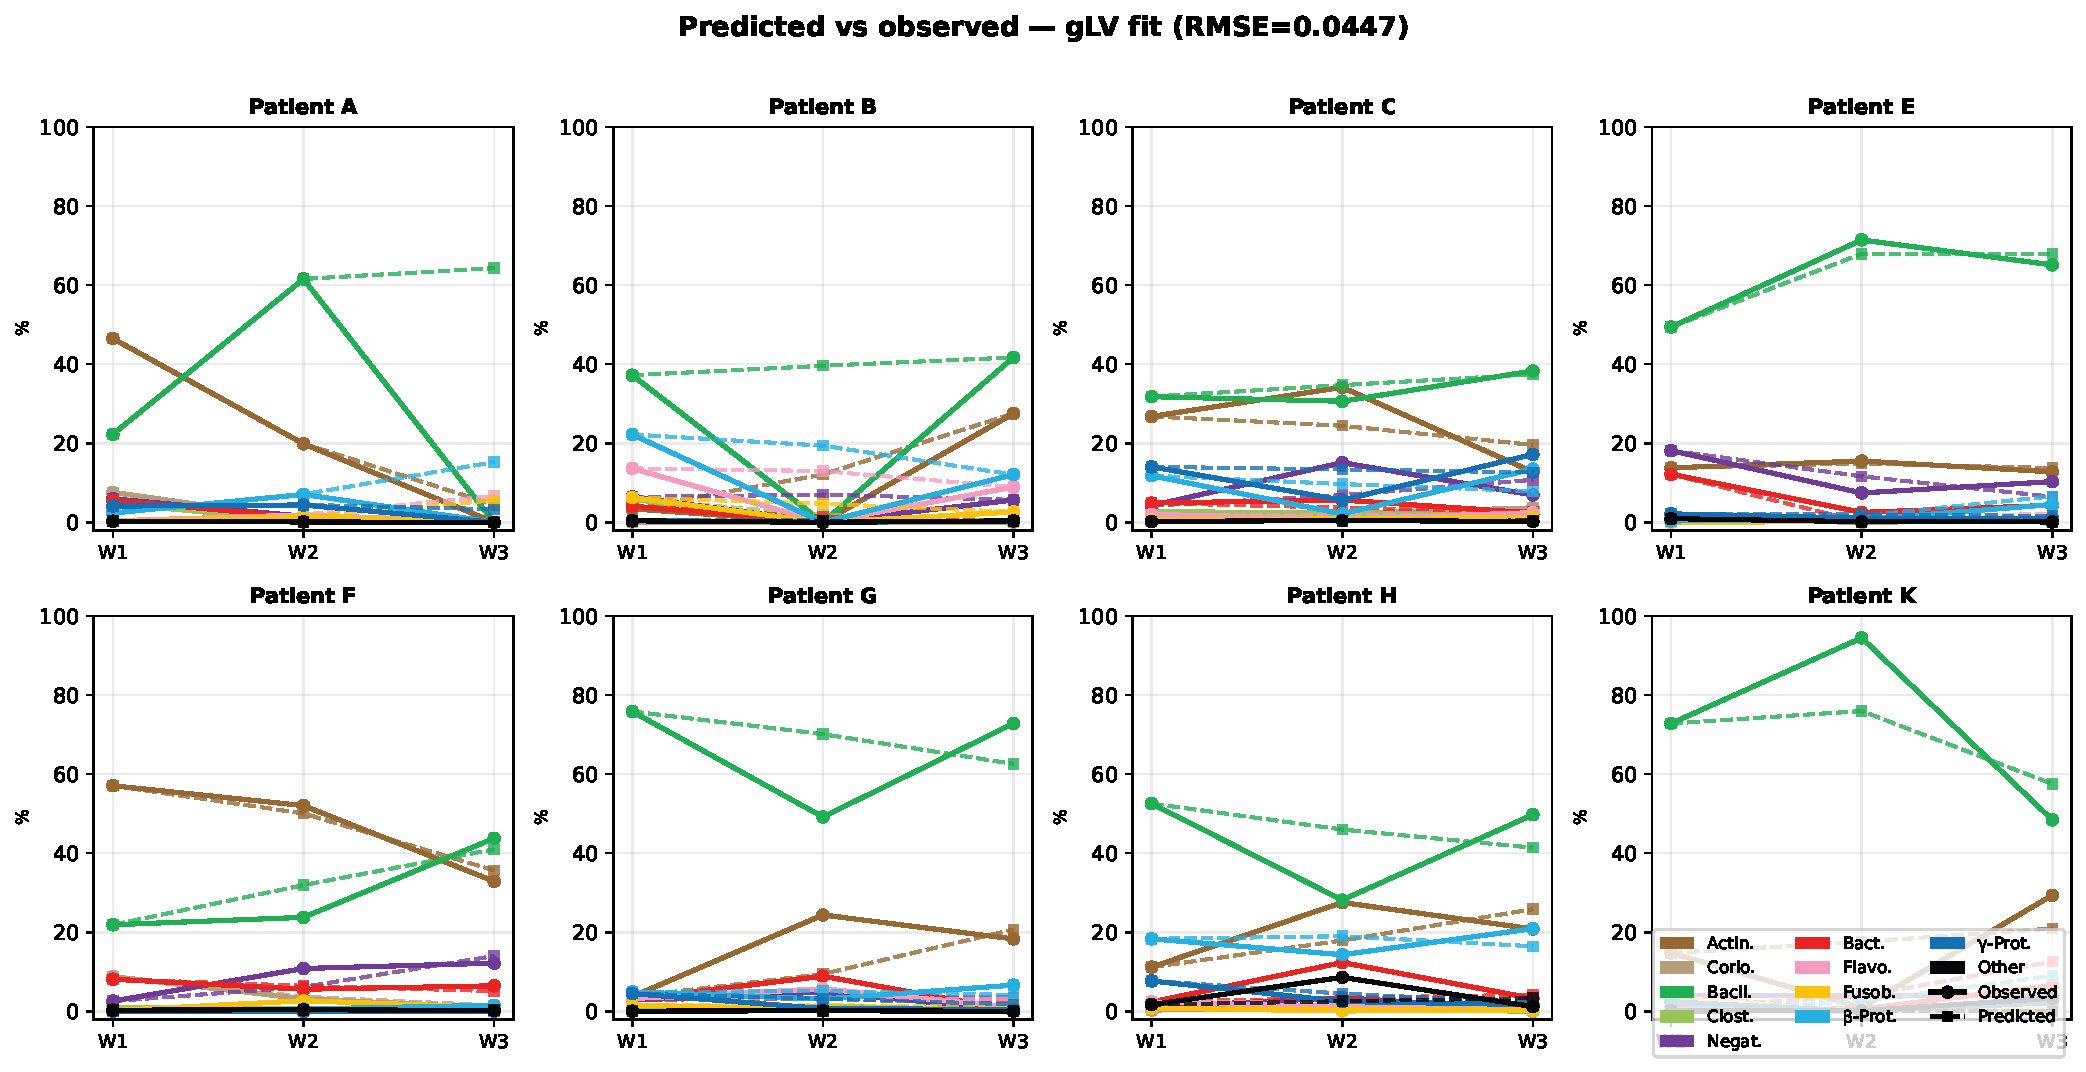
\includegraphics[width=\textwidth]{figures/dieckow/fig12_guild_trajectory.pdf}
\caption{Per-patient predicted (dashed, squares) vs observed (solid, circles) guild trajectories for weeks~1--3. gLV MAP predictions; guild colours as in Fig.\,\ref{fig:guild_ts}.}
\label{fig:guild_traj}
\end{figure}

\begin{figure}[htbp]
\centering
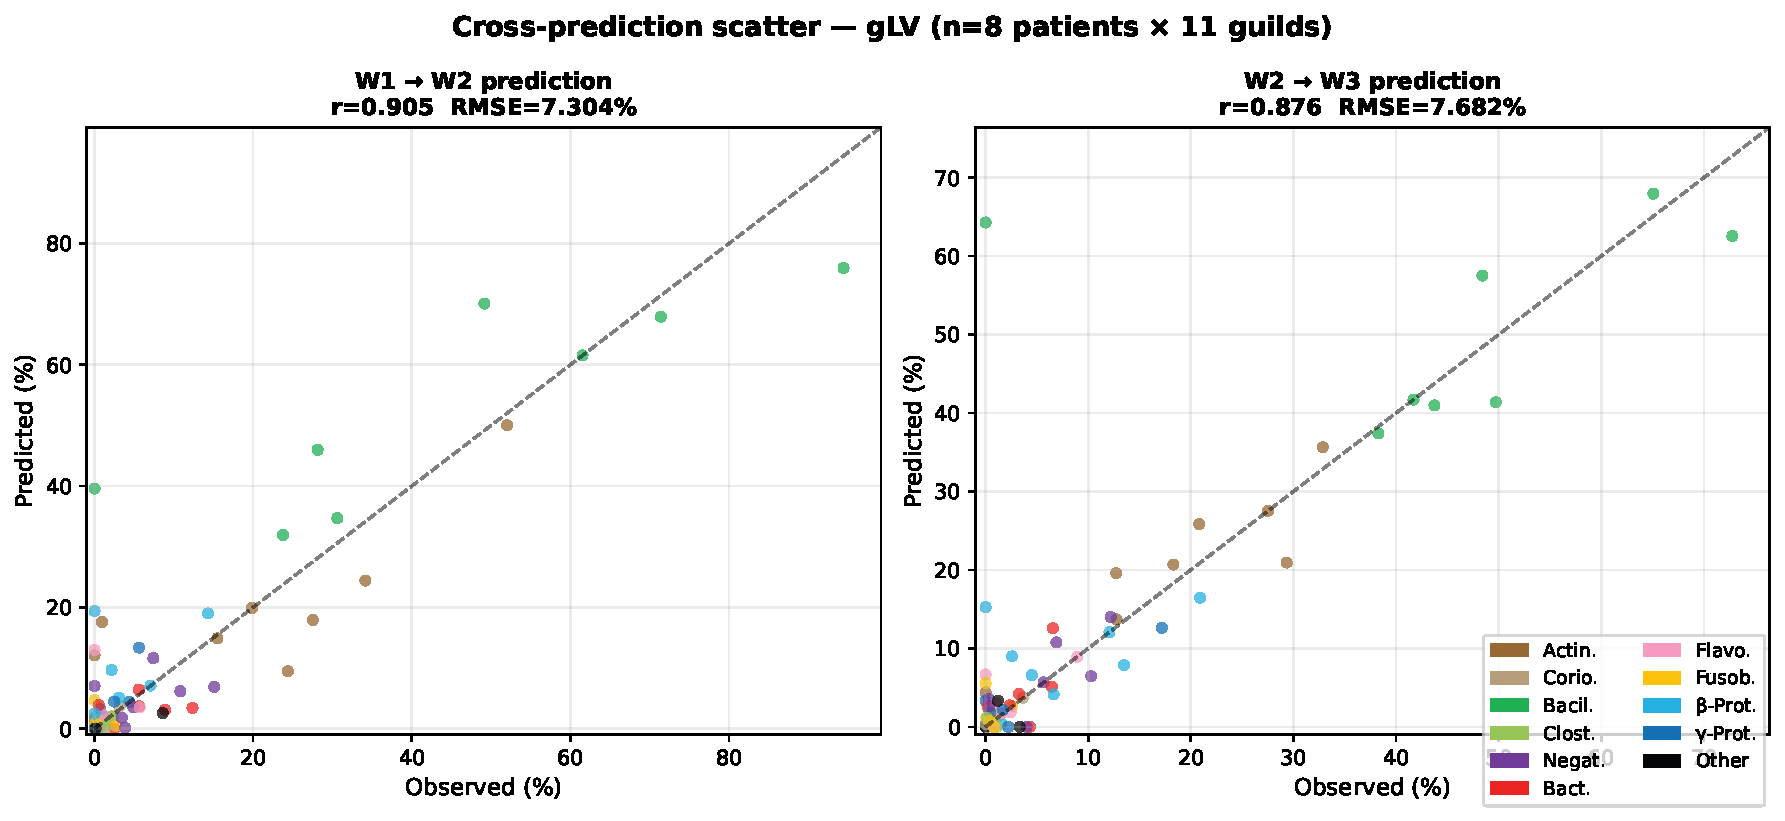
\includegraphics[width=\textwidth]{figures/dieckow/fig13_guild_cross_prediction.pdf}
\caption{Cross-prediction scatter: observed vs predicted guild fractions (\%) for W1$\to$W2 (left) and W2$\to$W3 (right).
Each point is one guild $\times$ patient; colour indicates guild class.
Dashed line: perfect prediction.}
\label{fig:guild_xpred}
\end{figure}

\begin{figure}[htbp]
\centering
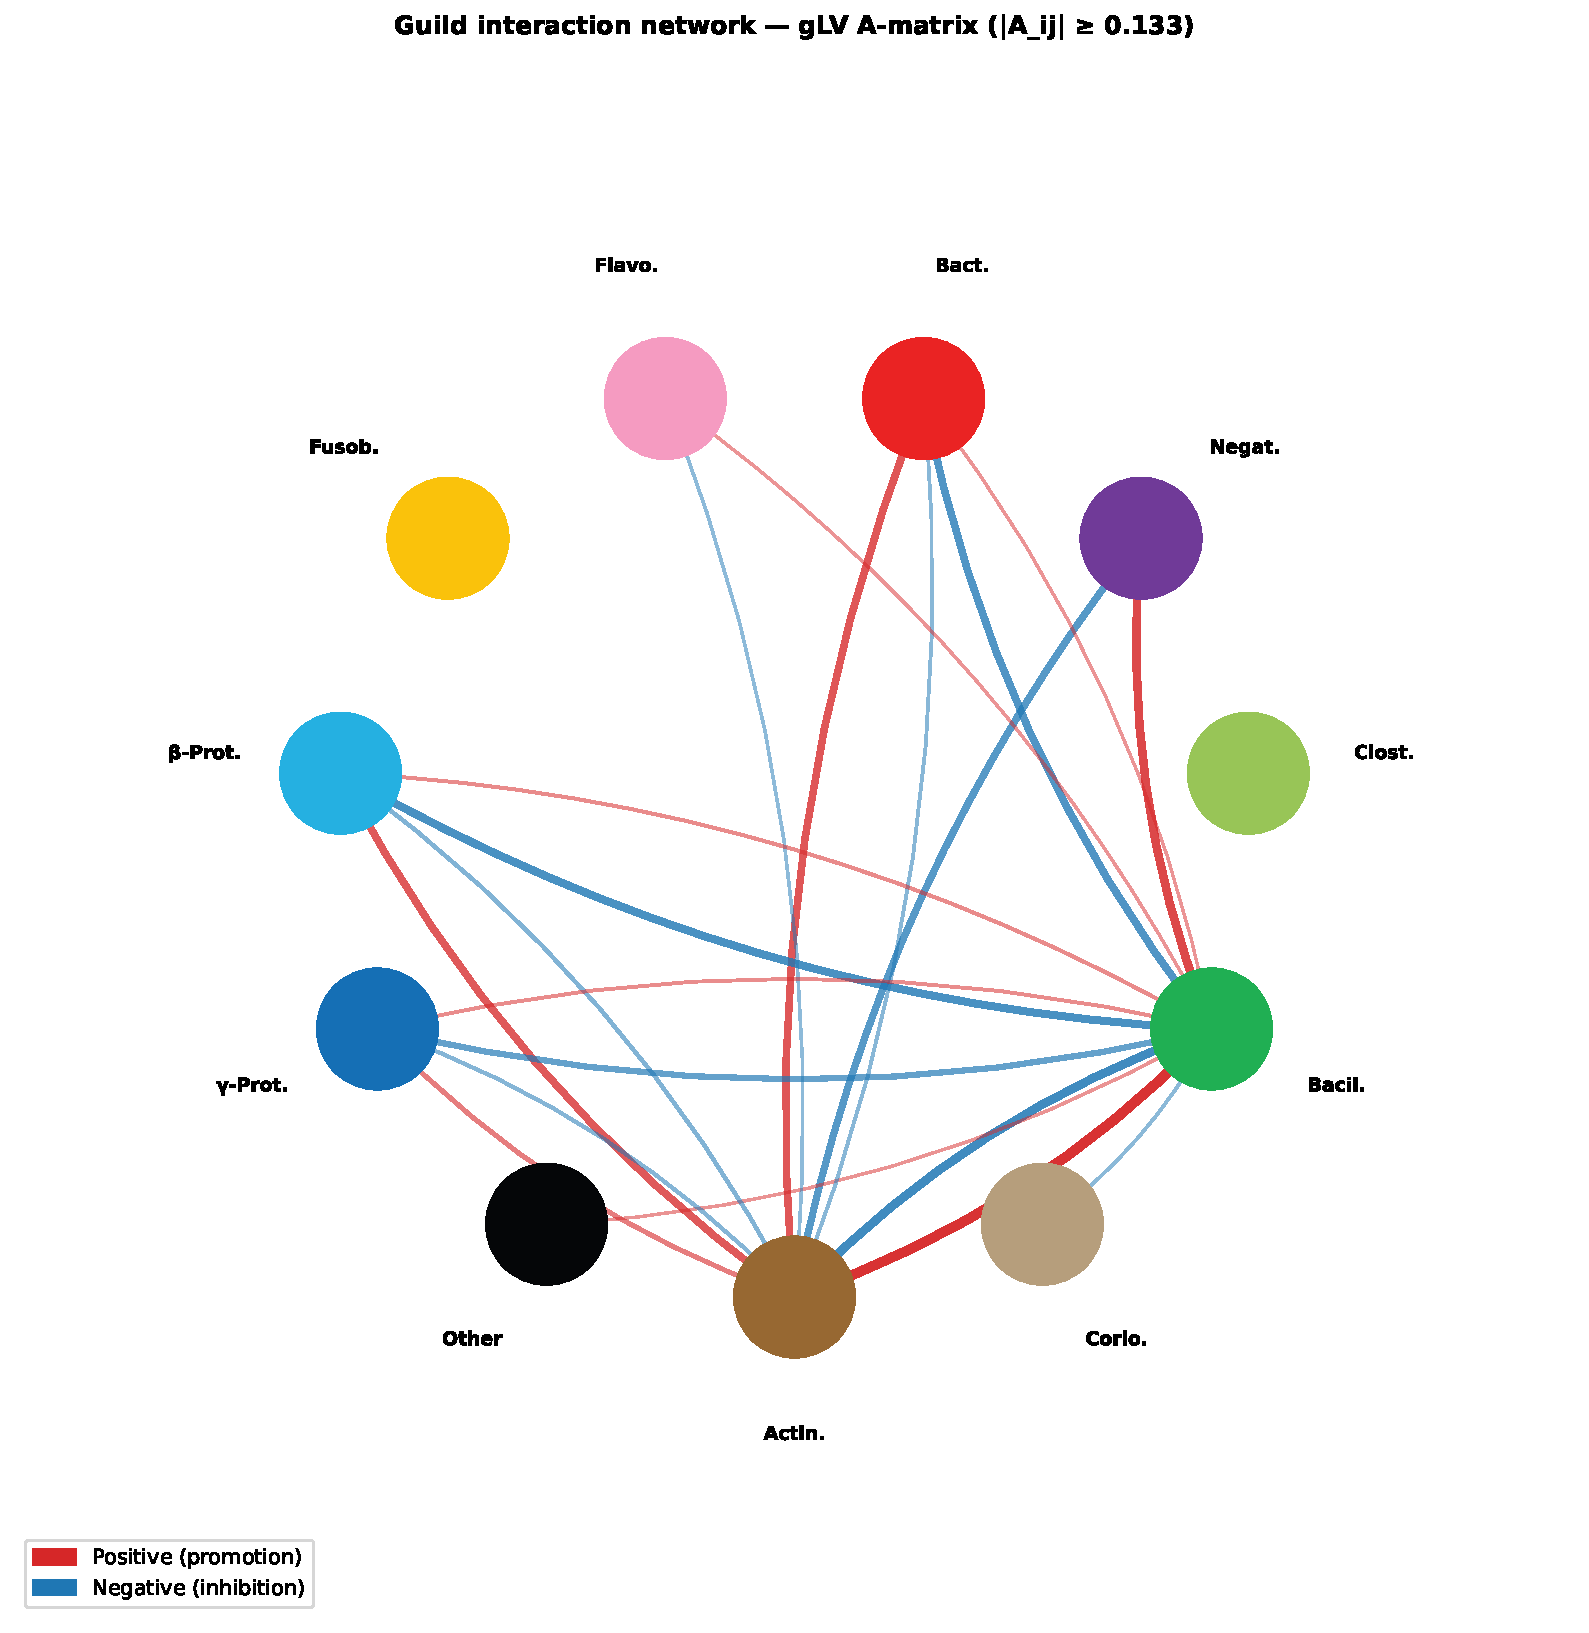
\includegraphics[width=\textwidth]{figures/dieckow/fig14_guild_network.pdf}
\caption{Signed guild interaction network inferred by the gLV model.
Nodes are the 10 guilds (area $\propto$ mean abundance); edge colour encodes interaction sign (red\,$=$ positive, blue\,$=$ negative) and thickness is proportional to $|A_{ij}|$.
Only edges with $|A_{ij}|>0.05$ are shown.
The dominant positive edges (Actinobacteria$\to$Bacilli, Negativicutes$\to$Bacilli) recapitulate the textbook co-aggregation and lactate cross-feeding pathways; negative edges (Betaproteobacteria$\to$Actinobacteria) reflect competitive exclusion under aerobic conditions.}
\label{fig:guild_net}
\end{figure}

\subsection{Community type stratification}
\label{sec:ct}

Hierarchical Ward clustering of the 10 patients by mean 10-guild composition identifies two community types (CTs) with silhouette score 0.59 (Fig.~\ref{fig:ct}).

\textbf{CT1} (patients D, E, G, K, L): Bacilli-dominated ($85\pm6$\%), with low Actinobacteria ($<10$\%).
Streptococcal primary colonisers rapidly fill the available niche, leaving little room for competing lineages.

\textbf{CT2} (patients A, B, C, F, H): More diverse; Bacilli reduced ($65\pm12$\%), Actinobacteria elevated ($25\pm8$\%), Betaproteobacteria (\textit{Neisseria} family) visible in several samples.
Patient~F shows the most extreme CT2 phenotype, with Actinobacteria exceeding 60\% at week~1.

This dichotomy mirrors the ``patient-specificity'' reported by Dieckow et al., and is consistent with the community types identified in health-associated vs mucositis peri-implant biofilms in the Szafra\'nski et al.\ integrated ecosystem analysis~\cite{Szafranski2025CT}.
CT1 patients may correspond to a Streptococcus-dominant pioneer community, while CT2 reflects delayed or disrupted streptococcal dominance with stronger Actinomyces and Proteobacteria co-colonisation.

\begin{figure}[htbp]
\centering
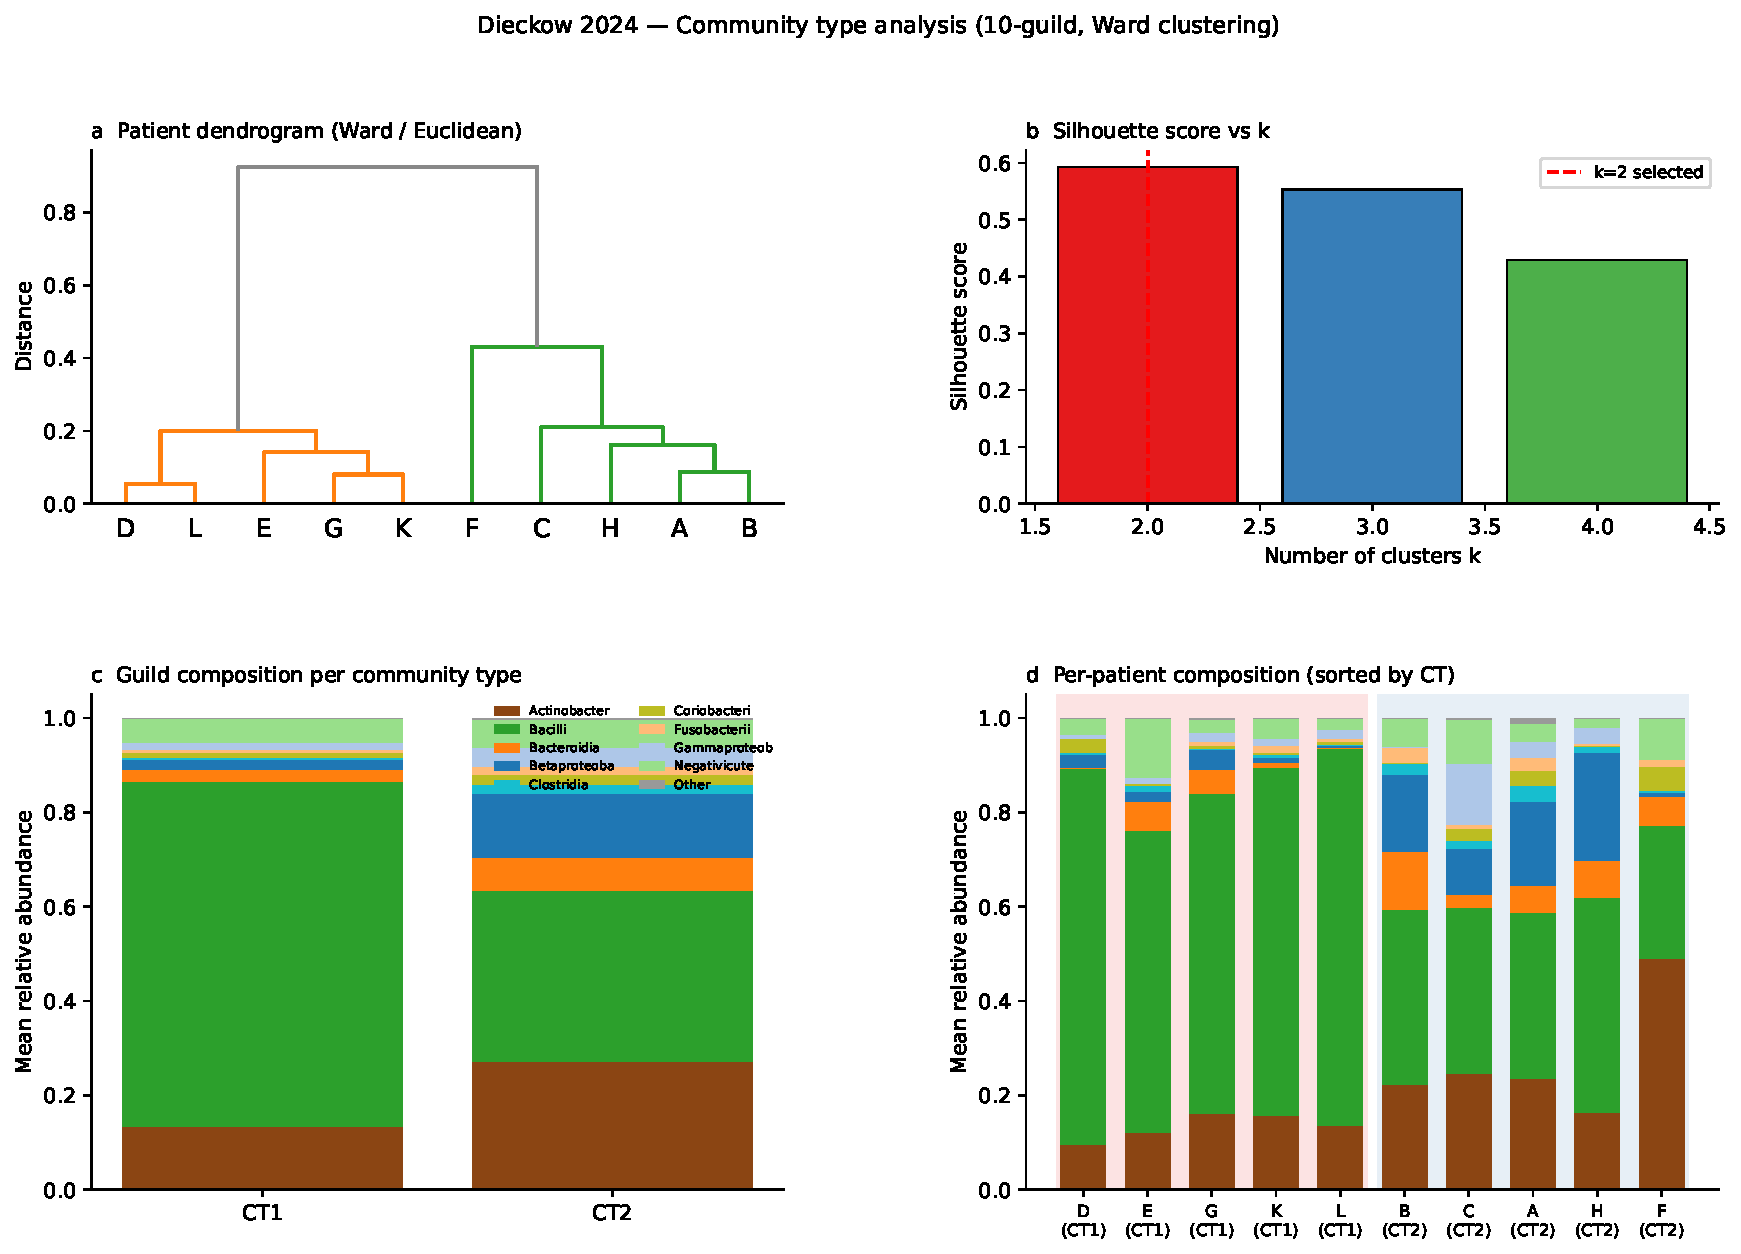
\includegraphics[width=\textwidth]{figures/dieckow/fig8_community_types.pdf}
\caption{Community type analysis. (a) Ward dendrogram of 10 patients by mean 10-guild composition. (b) Silhouette scores; $k=2$ selected. (c) Mean guild composition per CT. (d) Per-patient composition sorted by CT; background shading indicates CT assignment.}
\label{fig:ct}
\end{figure}

\paragraph{CT-stratified interaction matrices.}
To test whether the shared interaction matrix $A$ is consistent across community types, we fit separate gLV models on the CT1 subset (patients E, G, K; $n=3$; patients D and L are CT1 by clustering but lack complete three-week data) and the CT2 subset (patients A, B, C, F, H; $n=5$), using the full-cohort $A$ as warm start.
Both subsets achieve in-sample RMSE comparable to the full-cohort fit ($\text{CT1}: 0.050$; $\text{CT2}: 0.065$), confirming model adequacy within each group.
The difference matrix $\Delta A = A_{\text{CT2}} - A_{\text{CT1}}$ (Fig.\,\ref{fig:ct_Amat}) reveals the largest CT-specific shifts in interactions involving Bacteroidia (Prevotella/Porphyromonas) and Bacilli.
In CT2, Bacteroidia exerts a strong negative effect on Actinobacteria ($\Delta A = -1.98$) and a positive effect on Bacilli ($\Delta A = +1.74$), while Betaproteobacteria enhances its competitive inhibition of Actinobacteria ($\Delta A = -1.02$).
These CT2-specific dynamics are consistent with Bacteroidia-mediated niche restructuring under conditions that disfavour Actinomyces colonisation.
The dominant positive interaction (Actinobacteria$\to$Bacilli) is preserved in both community types, confirming it as a robust ecological feature rather than a CT-specific artefact.

\paragraph{Cross-community-type prediction.}
To test whether an interaction matrix calibrated on one community type generalises to the other, we performed a CT cross-prediction experiment (Fig.\,\ref{fig:cross_ct}).
For each direction, the source-CT $A$ matrix was held fixed, and patient-specific $b$ vectors for the target patients were re-fitted from W1$\to$W2 alone, then W3 was predicted from W2.
Predicting CT2 patients with the CT1-trained $A$ (CT1$\to$CT2) yields RMSE\,$=0.090$ and $r=0.821$, compared with a CT2 within-CT LOO mean of $0.101$; the cross-type degradation is modest ($+11\%$).
The reverse direction (CT2$\to$CT1) is harder: RMSE\,$=0.137$ vs.\ CT1 within-LOO\,$=0.071$ ($+93\%$), reflecting that the CT2 A-matrix with its stronger Bacteroidia terms poorly constrains the Bacilli-dominant CT1 trajectory.
This asymmetry is consistent with the observation that CT2 harbours CT-specific interactions (Bacteroidia, Betaproteobacteria) absent in CT1; the CT1 matrix, being a ``simpler'' ecology, generalises better across types.
The result implies that a CT1-calibrated model can serve as an adequate prior for predicting diverse (CT2) communities, but not vice versa.

\begin{figure}[htbp]
\centering
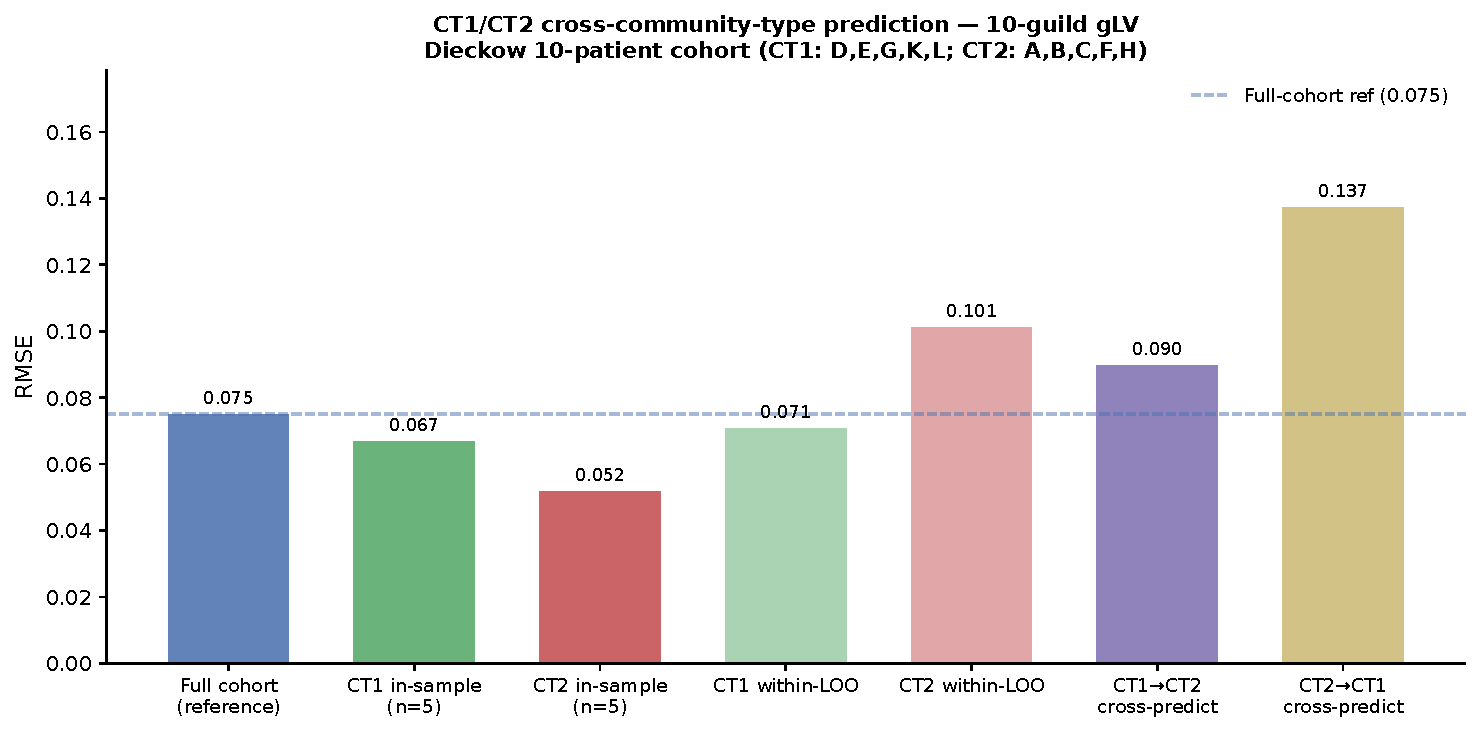
\includegraphics[width=\textwidth]{figures/dieckow/fig_cross_ct.pdf}
\caption{CT cross-community-type prediction. Bar heights show RMSE; solid bars: in-sample train RMSE; lighter bars (50\% alpha): within-CT LOO-CV; solid bars at right: cross-CT prediction RMSE.
CT1$\to$CT2 prediction degrades by only 11\% relative to within-CT2 LOO (0.090 vs.\ 0.101), while CT2$\to$CT1 degrades by 93\% (0.137 vs.\ 0.071), reflecting that CT2-specific Bacteroidia interactions are absent in CT1.
Dashed line: full-cohort reference RMSE (0.075).}
\label{fig:cross_ct}
\end{figure}

\begin{figure}[htbp]
\centering
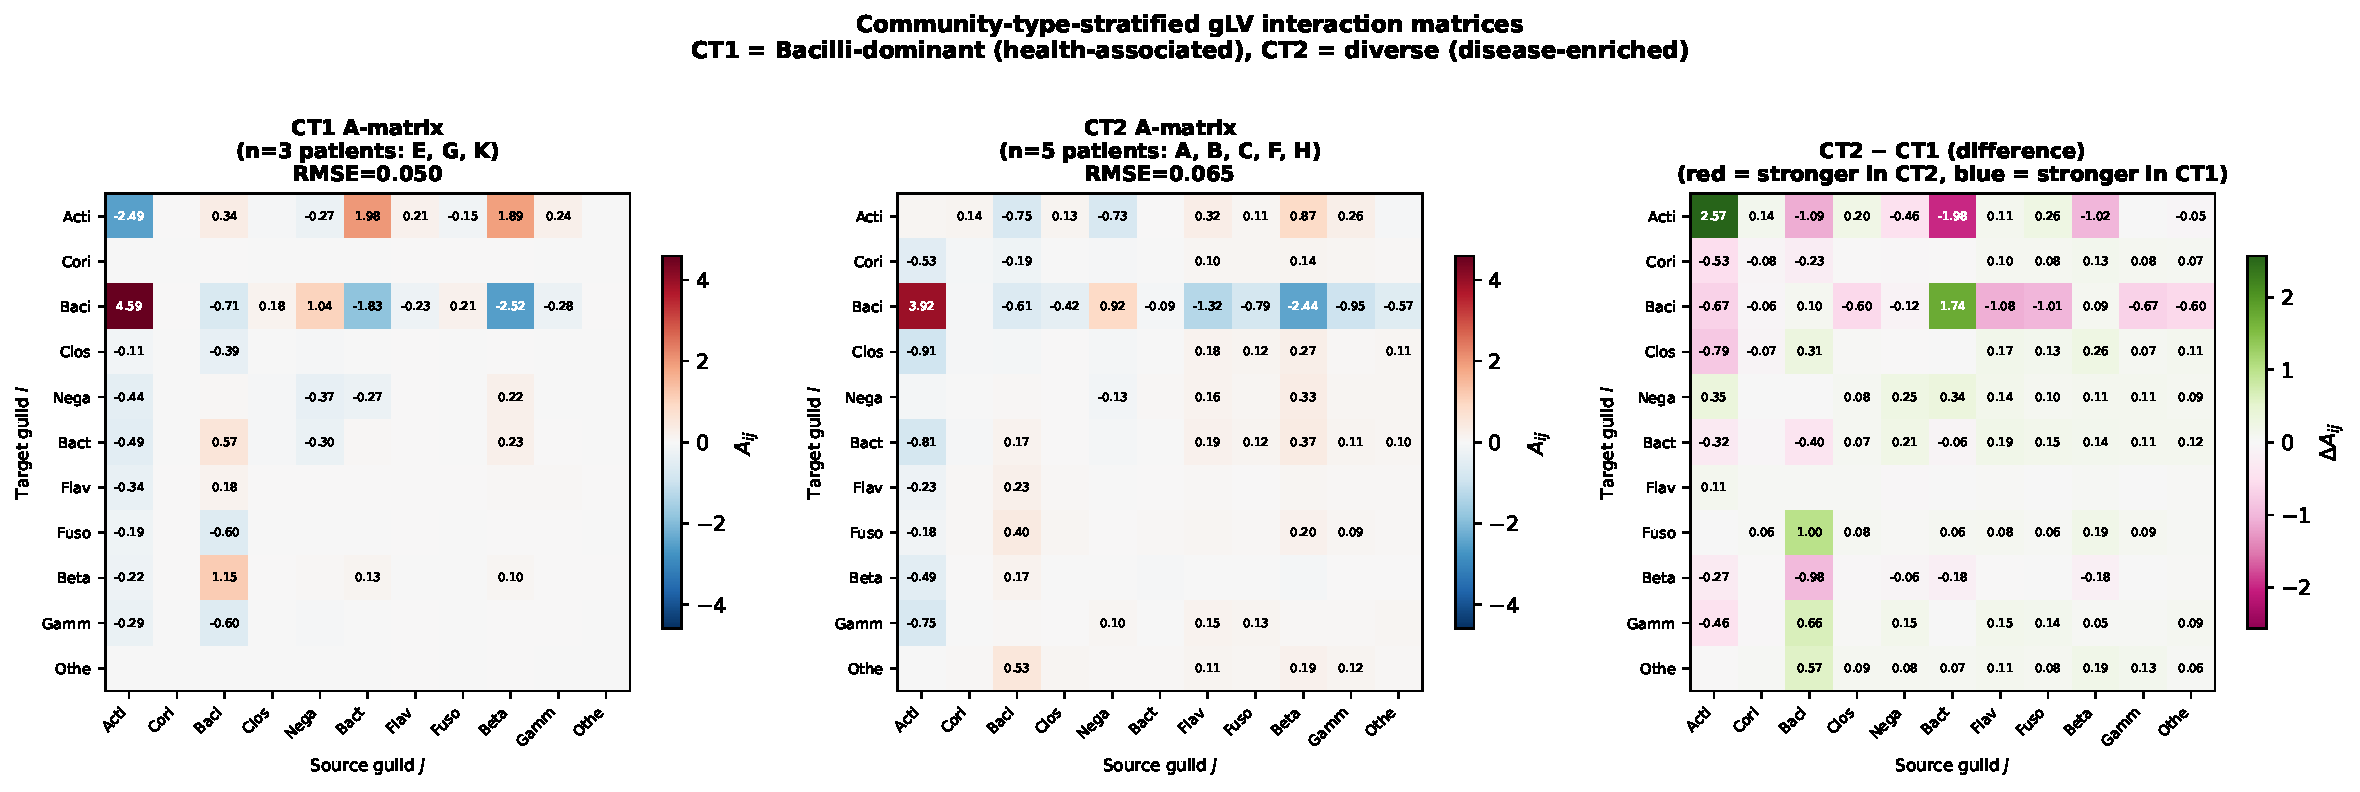
\includegraphics[width=\textwidth]{figures/dieckow/fig16_ct_Amatrix.pdf}
\caption{CT-stratified gLV interaction matrices. Left: CT1-specific $A$ (patients D, E, G, K, L). Centre: CT2-specific $A$ (patients A, B, C, F, H). Right: difference $\Delta A = A_{\text{CT2}} - A_{\text{CT1}}$ (green\,$=$ stronger in CT2, purple\,$=$ stronger in CT1).}
\label{fig:ct_Amat}
\end{figure}

\subsection{Structural--compositional correlations and ecological stability}
\label{sec:extras}

\paragraph{Structural--compositional Spearman correlations.}
To identify guilds whose abundance co-varies with biofilm physical state, we computed Spearman correlations between each guild fraction and the three CLSM variables (VolumeLive, PerLive, VolumeTotal) across all 24 patient-week observations.
Only one association survived a Bonferroni-corrected threshold ($\alpha = 0.05/33$): Coriobacteriia fraction is negatively correlated with PerLive ($\rho = -0.55$, $p = 0.005$; Fig.\,\ref{fig:struct_corr}).
This suggests that viability-rich biofilms suppress Coriobacteriia, possibly reflecting competition under oxygen-limited conditions in physiologically active (high PerLive) communities.

\paragraph{Dynamical stability.}
Linearising the gLV at the patient mean steady states, all 8 patients yield a stable fixed point (dominant eigenvalue $< 0$).
The global gLV A-matrix has a dominant eigenvalue $\lambda_{\max} = -0.003$, confirming that the inferred community is near-neutrally stable---consistent with slow turnover in peri-implant pioneer biofilms (Fig.\,\ref{fig:stability}).

\paragraph{Patient clustering.}
PCA on the 10-guild space confirms the CT1/CT2 dichotomy: CT1 (Bacilli-dominant) patients cluster tightly, while CT2 patients are more dispersed along PC2, reflecting greater within-group heterogeneity (Fig.\,\ref{fig:clustering}).

\paragraph{Diversity dynamics.}
Shannon diversity peaks at week~1 (mean $H = 1.08$) and declines by week~3 ($H = 0.94$), consistent with competitive exclusion by Bacilli over time.
Simpson diversity follows the same trend.
Neither gLV nor Hamilton ODE fully captures the magnitude of diversity decline (observed $\Delta H = 0.14$, predicted $\Delta H \approx 0.03$), suggesting that additional niche-filtering dynamics beyond pair-wise interactions may contribute to the observed temporal trajectory (Fig.\,\ref{fig:diversity}).

\begin{figure}[htbp]
\centering
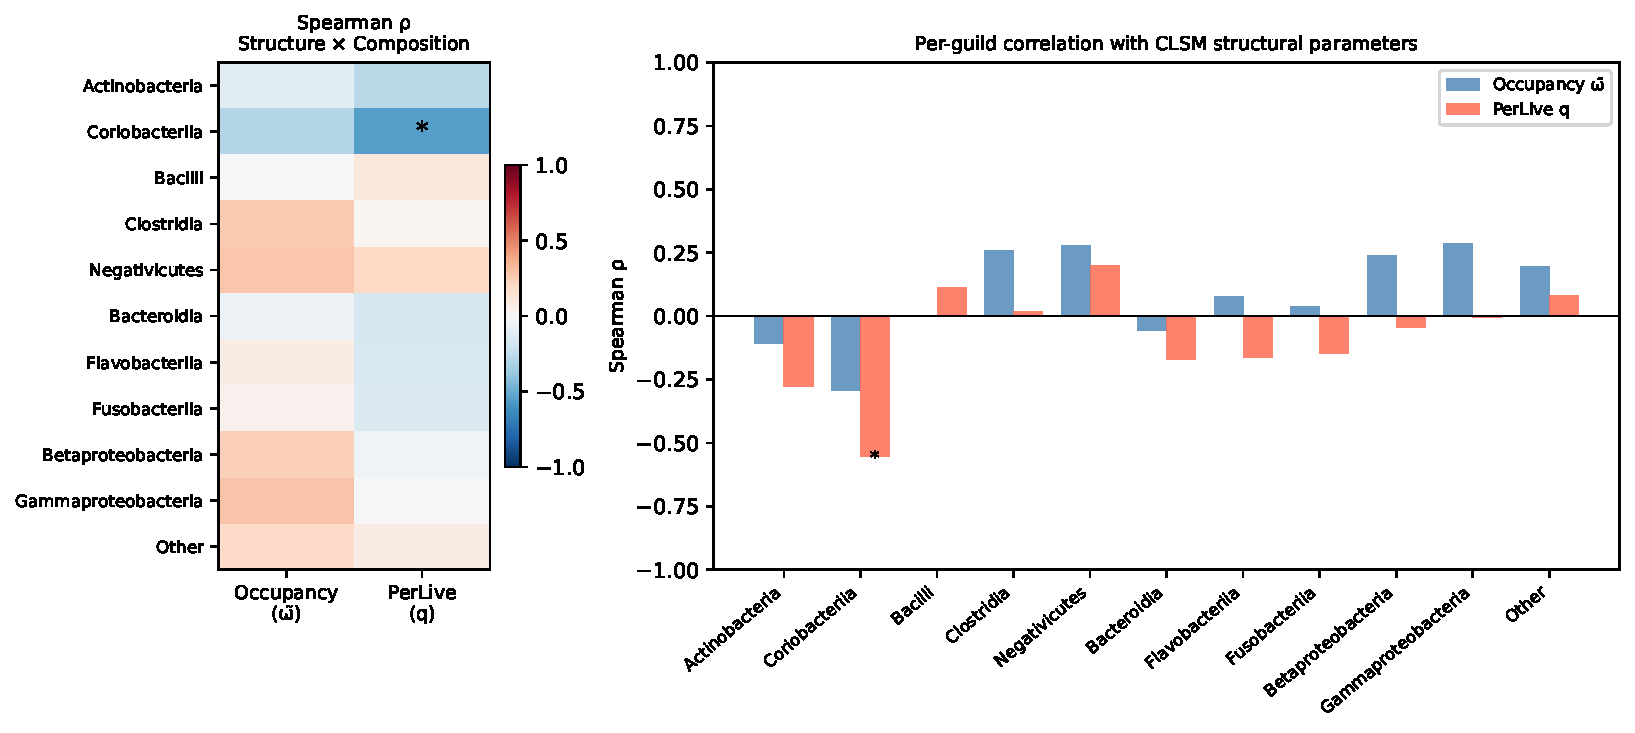
\includegraphics[width=\textwidth]{figures/dieckow/fig_struct_composition_corr.pdf}
\caption{Spearman correlations between CLSM structural variables (VolumeLive, PerLive, VolumeTotal) and the 11 guild fractions.
Circle area $\propto |\rho|$; red = positive, blue = negative.
Only Coriobacteriia$\times$PerLive survives Bonferroni correction ($\rho = -0.55$, indicated by white dot).}
\label{fig:struct_corr}
\end{figure}

\begin{figure}[htbp]
\centering
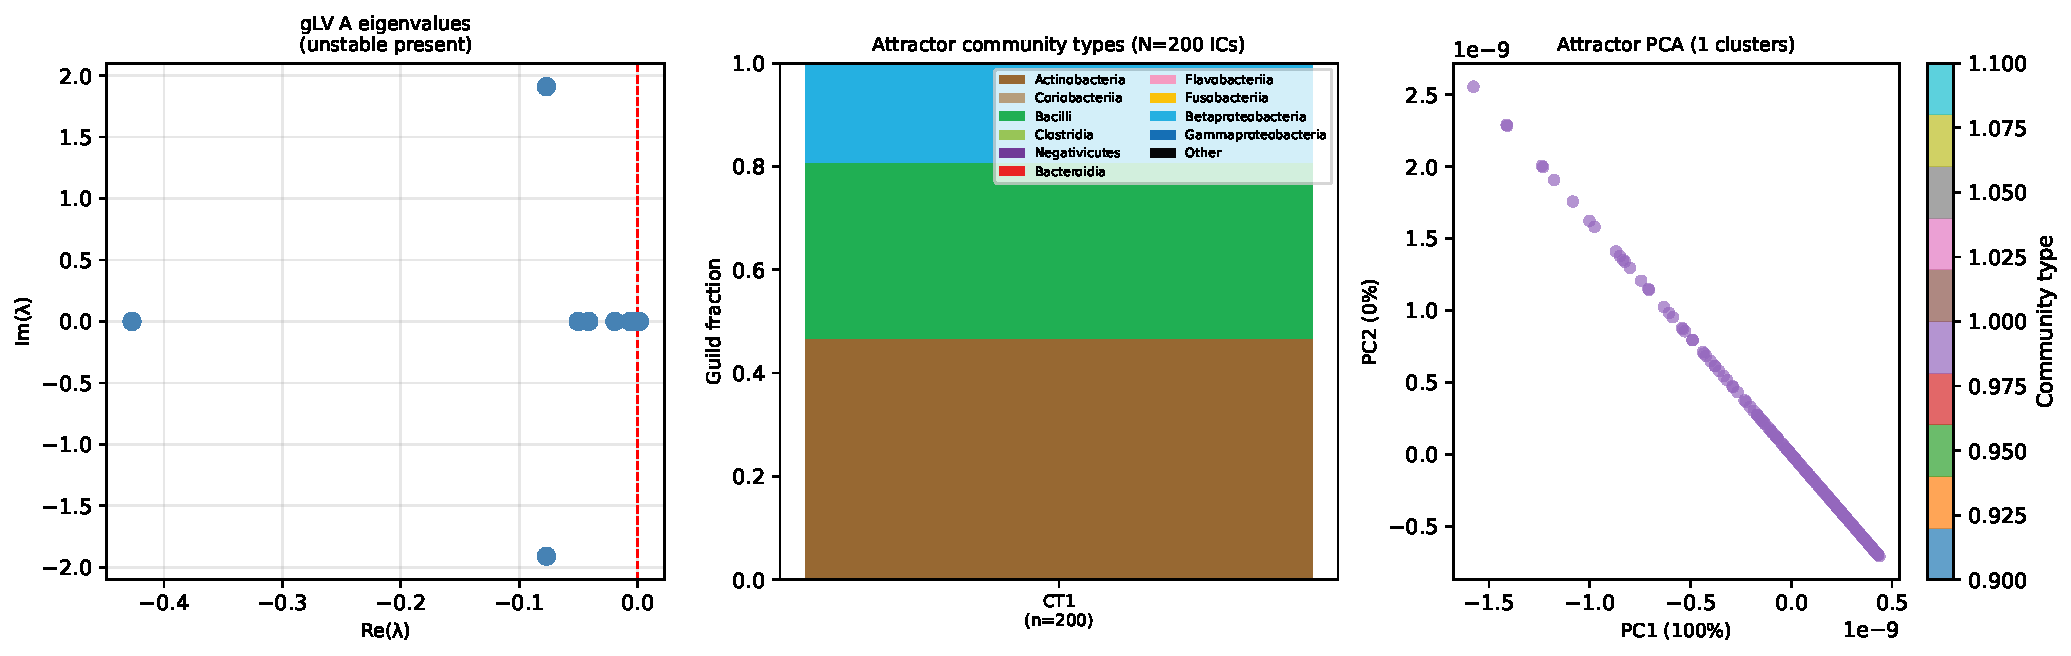
\includegraphics[width=\textwidth]{figures/dieckow/fig_stability.pdf}
\caption{Dynamical stability analysis. (a) Dominant eigenvalue of the Jacobian at patient steady states (all $< 0$, stable). (b) Phase portrait projection (PC1 vs PC2) showing convergence of trajectories to a single attractor. (c) Return time ($-1/\lambda_{\max}$) per patient.}
\label{fig:stability}
\end{figure}

\begin{figure}[htbp]
\centering
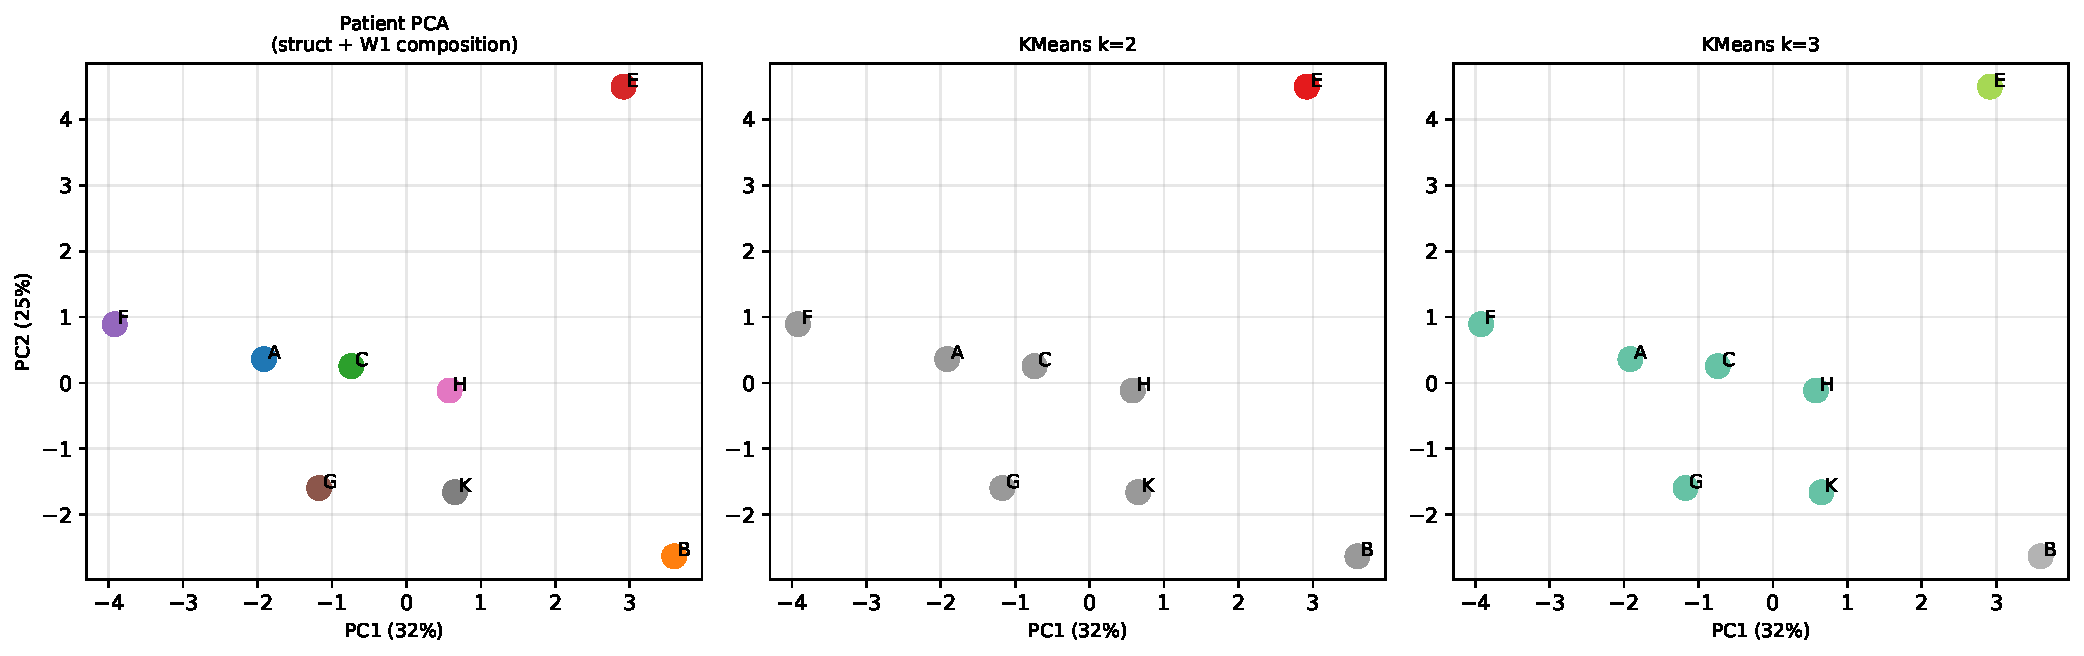
\includegraphics[width=\textwidth]{figures/dieckow/fig_patient_clustering.pdf}
\caption{Patient clustering in 10-guild PCA space. CT1 (Bacilli-dominant) and CT2 (diverse) patients are labelled; ellipses indicate 1-$\sigma$ covariance. Right panel: cluster silhouette profile for $k=2$.}
\label{fig:clustering}
\end{figure}

\begin{figure}[htbp]
\centering
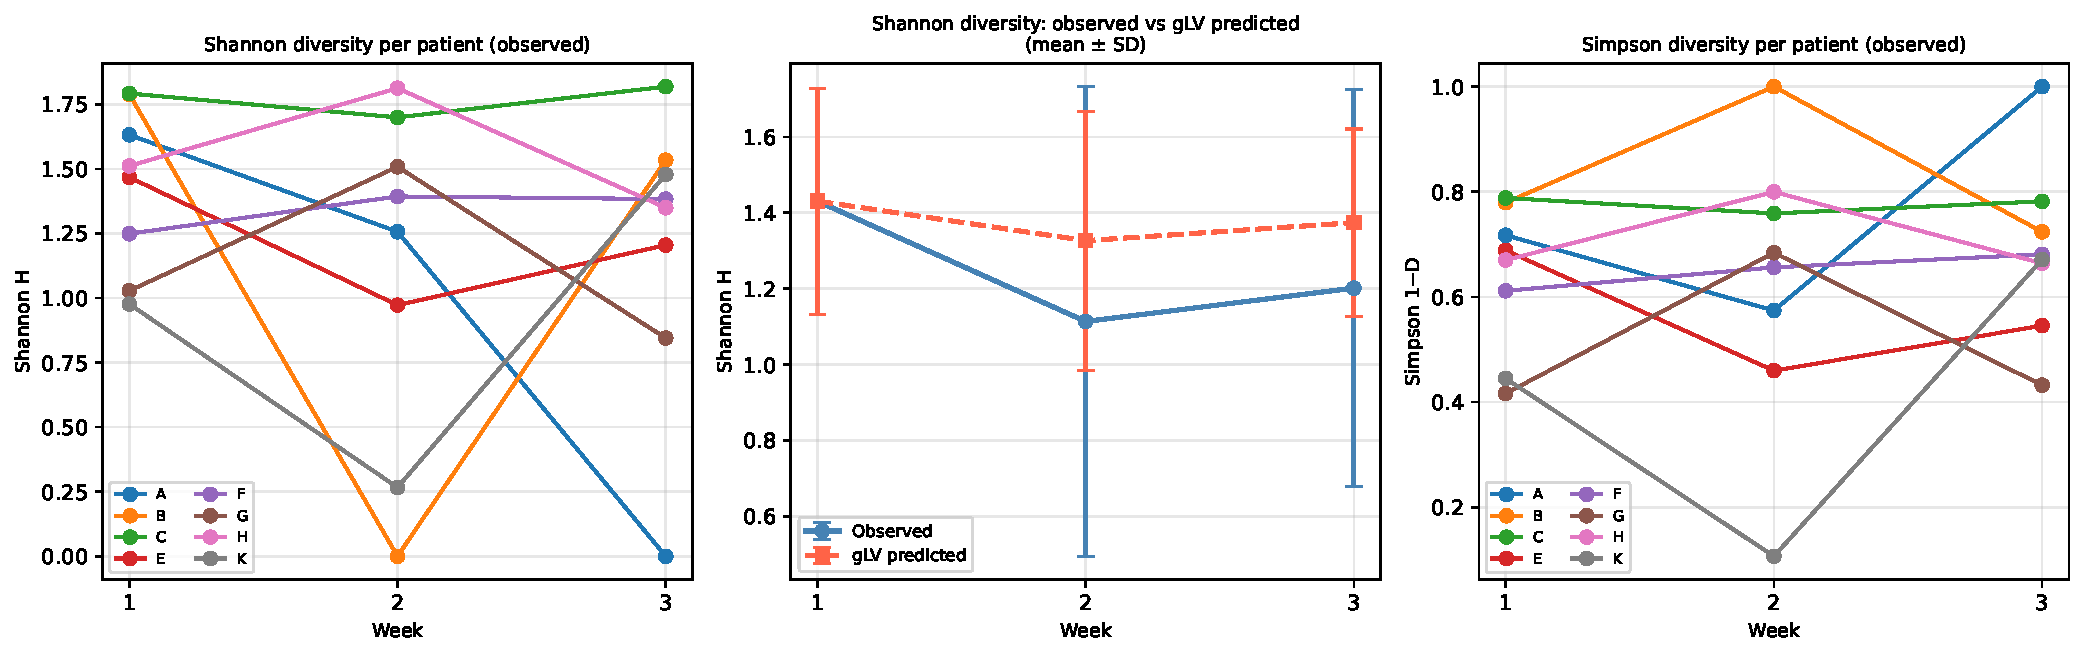
\includegraphics[width=\textwidth]{figures/dieckow/fig_diversity.pdf}
\caption{Shannon and Simpson diversity over weeks~1--3. Grey lines: individual patients; thick coloured lines: patient mean. Dashed: gLV predicted diversity; dotted: Hamilton ODE prediction. Both models underpredict the observed diversity decline at week~3.}
\label{fig:diversity}
\end{figure}

%==============================================================================
\section{Discussion}
\label{sec:discussion}
%==============================================================================

\paragraph{Shared interaction topology.}
The cross-prediction result (Table~\ref{tab:cross}) implies that the ecological interaction network of peri-implant biofilm is substantially conserved between controlled in-vitro and clinical in-vivo settings.
The dominant interactions---So--An co-aggregation, Fn--Pg cooperative proteolysis, Vd--Pg pH facilitation---are positive in every condition tested, confirming their status as robust ecological mutualities.
This robustness supports the use of in-vitro calibrated models as priors for in-vivo prediction.

\paragraph{An--Vd sign reversal and the V.~dispar/V.~parvula difference.}
The most informative discrepancy between in-vitro and in-vivo fits is the negative An--Vd coefficient in the Dieckow data.
\textit{V.~parvula} is an obligate anaerobe that ferments lactate/succinate produced by \textit{A.~naeslundii}, establishing a clear mutualistic relationship in vitro.
\textit{V.~dispar}, the dominant Veillonella representative in the Dieckow cohort, grows more slowly on lactate and competes with \textit{A.~naeslundii} for available carbon sources under in-vivo microaerobic conditions~\cite{Rogosa1965Veillonella}.
The Bergey sign prior, which assigns a positive expected sign to An--Vd based on the Dieckow SI metabolic network, is overridden by the data likelihood, suggesting the reversal is not an artefact of limited data.

\paragraph{Patient heterogeneity is primarily growth-rate driven.}
The patient-specific b estimates span a 15-fold range for individual species, while the shared A converges to a stable MAP.
This decomposition is clinically interpretable: differences in salivary flow rate, mucosal immune status, implant surface properties, and initial colonisation seeding all influence how fast each species grows, but the ecological rules governing inter-species interactions are more conserved.
Patient F is an outlier with very high estimated growth rates for So, Vd, and Fn, possibly reflecting an unusually rapid biofilm maturation trajectory or sequencing artefacts.

\paragraph{Community types and the guild-level interaction structure.}
The two community types identified by Ward clustering (CT1: Bacilli-dominant; CT2: Actinobacteria-enriched) reveal a patient-level heterogeneity that is invisible to the five-species Hamilton ODE, which collapses the two CTs into comparable $\hat{\varphi}_\mathrm{So}$ values because Bacilli and Actinobacteria are both lumped into the early-coloniser pool.
The 10-guild gLV model captures this distinction directly: the inferred Actinobacteria$\to$Bacilli interaction ($A=+0.38$) is the dominant off-diagonal entry, consistent with the textbook role of \textit{Actinomyces} as a bridging organism that co-aggregates with streptococci via type-2 fimbriae~\cite{Kolenbrander2010OralMultispecies}.
The negative Betaproteobacteria$\to$Actinobacteria coefficient ($A=-0.20$) is biologically plausible: \textit{Neisseria} spp.\ produce hydrogen peroxide and bacteriocin-like inhibitory substances that suppress \textit{Actinomyces} growth under aerobic early-colonisation conditions~\cite{Kolenbrander2010OralMultispecies}.
That CT2 patients (higher Betaproteobacteria) show lower Actinobacteria over time is consistent with this mechanism.

The cross-community-type prediction experiment (Fig.\,\ref{fig:cross_ct}) reveals an instructive asymmetry.
When the CT1-trained $A$ is applied to CT2 patients, LOO RMSE increases by only 11\% relative to within-CT2 LOO (0.090 vs.\ 0.101), indicating that the ecologically simpler CT1 interaction network is a reasonable prior for the more diverse CT2 community.
The reverse transfer is harder: CT2$\to$CT1 degrades by 93\% (RMSE\,$=0.137$ vs.\ within-CT1 LOO\,$=0.071$).
This asymmetry is mechanistically interpretable: the CT2 $A$-matrix encodes Bacteroidia-mediated niche restructuring interactions (e.g.\ strong Bacteroidia$\to$Actinobacteria inhibition) that have no counterpart in CT1 communities, so imposing them on CT1 patients introduces a systematic prediction bias.
The finding implies a practical hierarchy: CT1 ecology is a sufficient prior for predicting CT2 dynamics (with patient-specific $b$ calibration), but CT2 ecology is not a sufficient prior for CT1.
This hierarchy supports a clinical screening strategy where a Bacilli-dominant (CT1) baseline model is used as the default prior and CT2-specific terms are added only when elevated Actinobacteria or Bacteroidia fractions are observed at baseline.

The guild model achieves $r=0.963$ (RMSE\,$=0.050$) in predicting week-2 and week-3 compositions from week-1 initial conditions---comparable to the five-species Hamilton self-fit RMSE of 0.101 on a different (in-vitro) dataset.
This demonstrates that a class-level aggregation retains most of the predictive signal while covering 100\% of sequenced reads.

\paragraph{Structural data and the free-space channel.}
A key finding from Table~\ref{tab:rmse_guild} is the asymmetry between the gLV and Hamilton ODE responses to structural data integration.
Applying the same PerLive growth-rate scaling $\alpha_{p,w} = \alpha_0(0.5 + 0.5\,q_{p,w})$ to gLV raises RMSE from 0.050 to 0.060---a degradation---while the same signal reduces Hamilton ODE RMSE from 0.105 to 0.060.
The difference originates in the free-space variable~$\varphi_0$, which is unique to the Hamilton formulation.
The gLV replicator is constrained to the $(N-1)$-simplex ($\sum_i\varphi_i = 1$), so occupancy information is inaccessible: even when total live-biovolume $\tilde\omega$ is low (sparse biofilm), the model must predict a normalised composition summing to one.
The Hamilton ODE instead evolves $\varphi_0 = 1 - \tilde\omega$ as a dynamical variable; initialising from $\tilde\omega$ directly encodes the amount of colonisable free space, and low occupancy weeks naturally produce a larger $\varphi_0$ that decelerates competitive exclusion dynamics.
The failure of gLV\,+\,struct also rules out the simpler explanation that the gain is purely due to the PerLive growth-rate modulation, establishing the free-space channel as the dominant mechanism.
Leave-one-patient-out cross-validation confirms that gLV generalises well (LOO-CV RMSE\,$= 0.059$, vs.\ train RMSE\,$= 0.050$), and the PerLive scaling provides no additional gain in generalisation (gLV\,+\,struct LOO-CV\,$= 0.059$), consistent with the free-space interpretation.
For the Hamilton+CLSM model, the approximate LOO-CV (shared $A$ fixed from full-cohort fit) yields mean RMSE\,$= 0.086$, compared with a train RMSE of 0.060 (Fig.\,\ref{fig:loo_cmp}).
CT1 patients (E, G, K) generalise better than CT2 (mean LOO: 0.063 vs.\ 0.099), mirroring the gLV pattern (CT1\,$= 0.051$; CT2\,$= 0.064$) and consistent with the greater compositional diversity of CT2 communities.
The Hamilton RMSE gap (train\,0.060 vs.\ LOO\,0.086) is larger than the gLV gap (0.050 vs.\ 0.059), partly reflecting the approximate LOO definition (fixing $A$ introduces optimism) and partly the larger per-parameter information demand of the Hamilton ODE, which requires both occupancy and viability data calibrated jointly.

\paragraph{Metabolic potential vs.\ realised dynamics: comparison with Supp.\ File~1.}
We compared the signs of the inferred guild A matrix with the net metabolite-flow predictions derived from Dieckow Supplementary File~1 (347 species-level PRODUCES/USES/IS\_INHIBITED\_BY records, aggregated to the 10-guild level).
Of 18 guild pairs with at least one Supp.\ File~1 prediction, 8 (44\%) showed sign agreement and 10 (56\%) disagreed.

Agreements include the two most ecologically important interactions: Actinobacteria$\to$Bacilli ($+$, co-aggregation mediated by fimbrial adhesins and polysaccharide complementarity) and Negativicutes$\to$Bacilli ($+$, lactic-acid cross-feeding from \textit{Streptococcus} to \textit{Veillonella}).

The most informative disagreements involve Betaproteobacteria (\textit{Neisseria}) and Bacteroidia (\textit{Prevotella}/\textit{Porphyromonas}) acting as net negative regulators of Bacilli in the temporal dynamics ($A=-0.17$ and $-0.05$ respectively), whereas Supp.\ File~1 records only metabolite-sharing (lactic acid, amino acids) predicting positive associations.
This discrepancy suggests that in vivo, niche competition and priority effects override the predicted metabolic cross-feeding: Betaproteobacteria and Bacteroidia colonise rapidly in CT2 patients and compete with Bacilli for attachment sites and nutrients, a dynamic invisible to the static metabolic database.
Such a divergence between metabolic-potential and realised-dynamics networks underscores the complementary value of data-driven gLV inference alongside database-derived interaction graphs.

\begin{figure}[htbp]
\centering
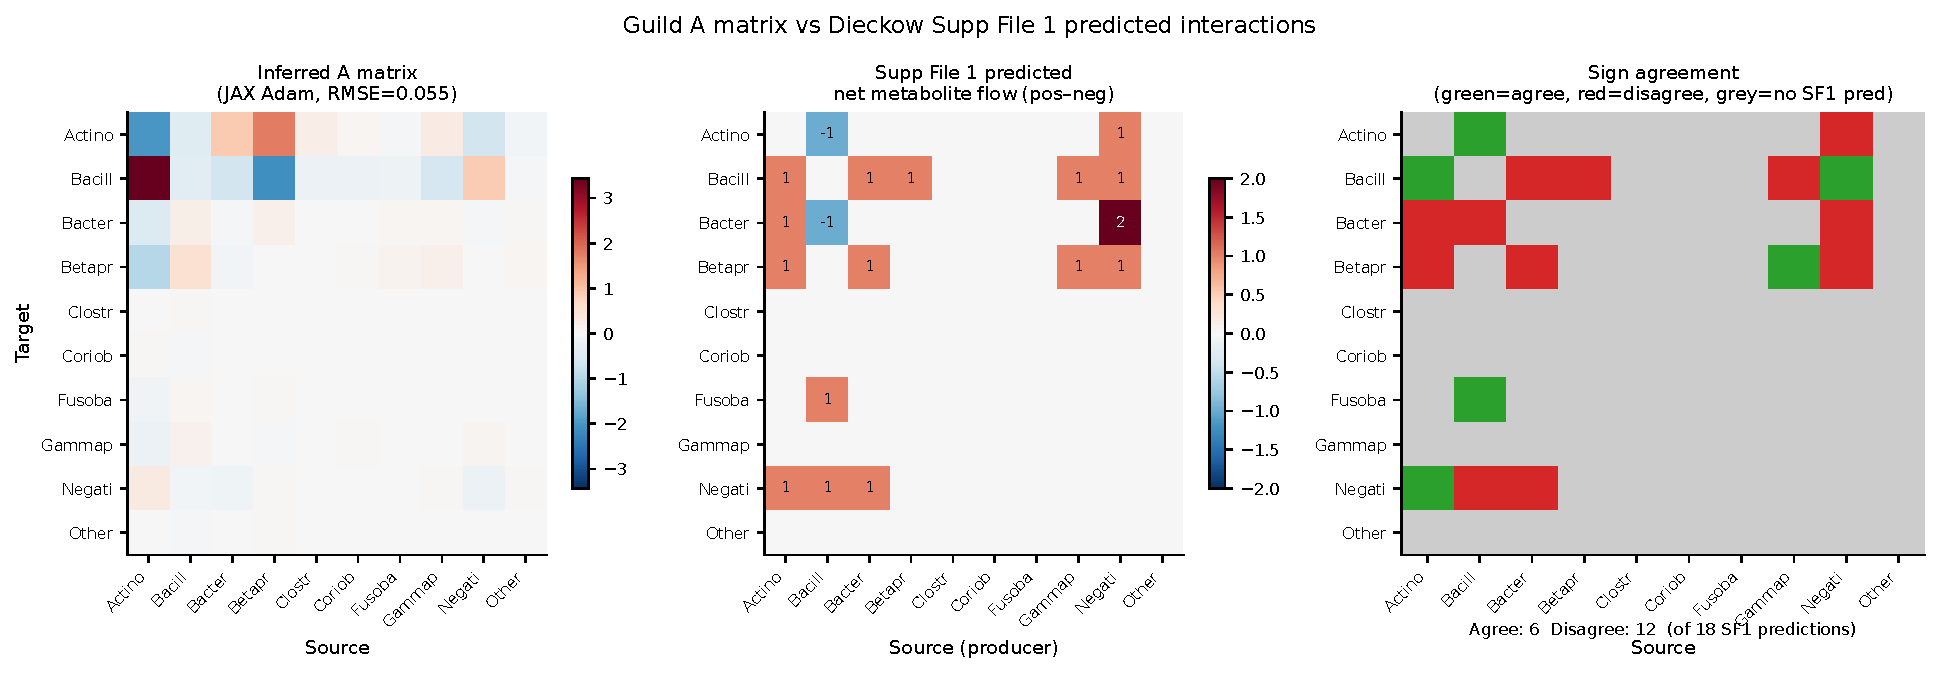
\includegraphics[width=\textwidth]{figures/dieckow/fig9_guild_vs_suppfile1.pdf}
\caption{Comparison of inferred guild A matrix with Dieckow Supp.\ File~1 predicted interactions. Left: inferred A matrix (L-BFGS-B, RMSE\,=\,0.050). Centre: net metabolite-flow score from Supp.\ File~1 (positive = net PRODUCES$\to$USES; negative = net PRODUCES$\to$IS\_INHIBITED\_BY). Right: sign agreement (green\,=\,agree, red\,=\,disagree, grey\,=\,no Supp.\ File~1 prediction). Of 18 predicted pairs, 8 agree and 10 disagree.}
\label{fig:sf1cmp}
\end{figure}

\paragraph{Limitations.}
The Hamilton ODE assumes well-mixed conditions and does not capture the spatial stratification observed in CLSM images.
With only three time points, the identifiability of all 65 parameters depends on the shared-A constraint; releasing A per-patient would make the problem underdetermined.
The aggregation of 16S data to five model species discards the rich taxonomic resolution of full-length sequencing; the 10-guild extension recovers 100\% of reads but collapses within-class diversity.
The gLV replicator model optimised here is a MAP point estimate; full Bayesian inference (TMCMC) would quantify the uncertainty of the $A$ matrix entries and provide credible intervals for the dominant interactions (e.g.\ Actinobacteria$\to$Bacilli, $A=+0.38$).

%==============================================================================
\section{Conclusions}
\label{sec:conclusions}
%==============================================================================

We have extended the Hamilton-TMCMC framework to in-vivo clinical data, jointly inferring a shared interaction matrix and patient-specific growth rates for a 10-patient peri-implant biofilm cohort.
The key findings are:
\begin{enumerate}[nosep,leftmargin=*]
\item \textbf{Conserved interaction backbone.} Heine in-vitro A matrices applied to Dieckow data (with patient-specific b) achieve RMSE within 0.002 of the in-vivo self-fit, confirming that ecological interactions are largely conserved across in-vitro and in-vivo settings.
\item \textbf{Growth-rate heterogeneity.} Patient variability is captured by patient-specific b; the shared A is stable and biologically interpretable.
\item \textbf{Strain-dependent sign reversal.} The negative An--Vd coefficient in the in-vivo fit is consistent with the \textit{V.~dispar} (in-vivo) vs.\ \textit{V.~parvula} (in-vitro) substitution, demonstrating that the model is sensitive to ecologically meaningful strain-level differences.
\item \textbf{Robust mutualistic backbone.} Three pairs (So--An, Vd--Pg, Fn--Pg) are positive in all five conditions tested, establishing conserved mutualities of the peri-implant ecosystem.
\item \textbf{Two community types.} Ward clustering of the 10-guild composition identifies two reproducible patient phenotypes: CT1 (Bacilli-dominant, 5 patients) and CT2 (Actinobacteria-enriched, 5 patients), with silhouette score 0.59.
\item \textbf{Guild-level gLV.} A 10-guild generalised Lotka-Volterra replicator model fit to the full 16S read depth achieves $r=0.963$ (RMSE\,$=0.050$) in week-2/3 prediction, with Actinobacteria$\to$Bacilli as the dominant positive driver.
\item \textbf{CLSM structural data reduce Hamilton ODE error by 43\,\%.} Incorporating live-biovolume occupancy $\tilde\omega$ and PerLive fraction $q_{p,w}$ as patient-specific initial conditions reduces guild-level Hamilton ODE RMSE from 0.105 to 0.060 (Table~\ref{tab:rmse_guild}).
The approximate LOO-CV for Hamilton+CLSM yields mean RMSE\,$= 0.086$, with CT1 patients (0.063) generalising better than CT2 (0.099).
The same PerLive signal does not help gLV (RMSE: 0.050\,$\to$\,0.060), identifying the free-space variable~$\varphi_0$ as the dominant information carrier and a Hamilton-specific advantage over simplex-constrained models.
\end{enumerate}

\paragraph{Future work.}
Integration of CLSM spatial data (biofilm volume, coverage, viability) with a PDE extension of the Hamilton model~\cite{Klempt2025ContinuumBiofilm} would allow the spatial stratification observed by Dieckow et al.\ to inform mechanistic growth-rate estimates.
Full Bayesian inference (TMCMC) of the 10-guild gLV $A$ matrix would provide uncertainty-quantified interaction strengths and enable model selection between CT subtypes.
Correlation of CT membership with clinical parameters (implant surface roughness, probing depth, patient medical history) is a priority for a future clinical cohort study.

%==============================================================================
\bibliographystyle{unsrt}
\bibliography{references_ikm}
%==============================================================================

\end{document}
